%Version 2.1 April 2023
%DIF LATEXDIFF DIFFERENCE FILE
%DIF DEL endo_stoch_demo_EcolLetters.tex            Tue Feb 20 09:44:17 2024
%DIF ADD endo_stoch_demo_EcolLetters_revision.tex   Tue Feb 20 09:45:17 2024
% See section 11 of the User Manual for version history
%
%%%%%%%%%%%%%%%%%%%%%%%%%%%%%%%%%%%%%%%%%%%%%%%%%%%%%%%%%%%%%%%%%%%%%%
%%                                                                 %%
%% Please do not use \input{...} to include other tex files.       %%
%% Submit your LaTeX manuscript as one .tex document.              %%
%%                                                                 %%
%% All additional figures and files should be attached             %%
%% separately and not embedded in the \TeX\ document itself.       %%
%%                                                                 %%
%%%%%%%%%%%%%%%%%%%%%%%%%%%%%%%%%%%%%%%%%%%%%%%%%%%%%%%%%%%%%%%%%%%%%

%%\documentclass[referee,sn-basic]{sn-jnl}% referee option is meant for double line spacing

%%=======================================================%%
%% to print line numbers in the margin use lineno option %%
%%=======================================================%%

\documentclass[lineno,sn-nature]{sn-jnl}% Basic Springer Nature Reference Style/Chemistry Reference Style

%%======================================================%%
%% to compile with pdflatex/xelatex use pdflatex option %%
%%======================================================%%

%%\documentclass[pdflatex,sn-basic]{sn-jnl}% Basic Springer Nature Reference Style/Chemistry Reference Style


%%Note: the following reference styles support Namedate and Numbered referencing. By default the style follows the most common style. To switch between the options you can add or remove “Numbered” in the optional parenthesis. 
%%The option is available for: sn-basic.bst, sn-vancouver.bst, sn-chicago.bst, sn-mathphys.bst. %  
%% \documentclass[sn-nature]{sn-jnl}% Style for submissions to Nature Portfolio journals
%%\documentclass[sn-basic]{sn-jnl}% Basic Springer Nature Reference Style/Chemistry Reference Style
%%\documentclass[sn-mathphys,Numbered]{sn-jnl}% Math and Physical Sciences Reference Style
%%\documentclass[sn-aps]{sn-jnl}% American Physical Society (APS) Reference Style
%%\documentclass[sn-vancouver,Numbered]{sn-jnl}% Vancouver Reference Style
%%\documentclass[sn-apa]{sn-jnl}% APA Reference Style 
%%\documentclass[sn-chicago]{sn-jnl}% Chicago-based Humanities Reference Style
%%\documentclass[default]{sn-jnl}% Default
%%\documentclass[default,iicol]{sn-jnl}% Default with double column layout

%%%% Standard Packages
%%<additional latex packages if required can be included here>

\usepackage{graphicx}%
\usepackage{multirow}%
\usepackage{amsmath,amssymb,amsfonts}%
\usepackage{amsthm}%
\usepackage{mathrsfs}%
\usepackage[title]{appendix}%
\usepackage{xcolor}%
\usepackage{textcomp}%
\usepackage{manyfoot}%
\usepackage{booktabs}%
\usepackage{algorithm}%
\usepackage{algorithmicx}%
\usepackage{algpseudocode}%
\usepackage{listings}%
\usepackage{natbib}
\usepackage{totcount}
\usepackage{soul}

\providecommand{\DIFadd}[1]{{\protect\color{blue}#1}} %DIF PREAMBLE
\providecommand{\DIFdel}[1]{{\protect\color{red}\protect\scriptsize\sout{#1}}}



%%%%

%%%%%=============================================================================%%%%
%%%%  Remarks: This template is provided to aid authors with the preparation
%%%%  of original research articles intended for submission to journals published 
%%%%  by Springer Nature. The guidance has been prepared in partnership with 
%%%%  production teams to conform to Springer Nature technical requirements. 
%%%%  Editorial and presentation requirements differ among journal portfolios and 
%%%%  research disciplines. You may find sections in this template are irrelevant 
%%%%  to your work and are empowered to omit any such section if allowed by the 
%%%%  journal you intend to submit to. The submission guidelines and policies 
%%%%  of the journal take precedence. A detailed User Manual is available in the 
%%%%  template package for technical guidance.
%%%%%=============================================================================%%%%

%\jyear{2021}%

\raggedbottom
%%\unnumbered% uncomment this for unnumbered level heads


%%=====================================================%%
%% redefining the title page to include author contributions
\makeatletter
\newcommand\@contrib{}%
\newcommand\@availab{}%


\def\statementsheadfont{\reset@font\fontsize{7bp}{9.5bp}\bfseries\selectfont\titraggedcenter}%
\def\statementssubheadfont{\reset@font\fontsize{7bp}{9.5bp}\bfseries\selectfont}%
\def\statementsfont{\reset@font\fontsize{7bp}{9.5bp}\selectfont\leftskip=24pt\rightskip=24pt\parfillskip=0pt plus 1fil}%




\newcommand\contribhead{\@startsection {section}{1}{\z@}{-22pt \@plus0ex \@minus0ex}{3pt}{\statementsheadfont}}%
\newcommand\contribsubhead{\@startsection{subsection}{2}{\z@}{3pt \@plus0ex \@minus0ex}{-.5em}{\statementssubheadfont}}

\newcommand\availabhead{\@startsection {section}{1}{\z@}{-22pt \@plus0ex \@minus0ex}{3pt}{\statementsheadfont}}%
\newcommand\availabsubhead{\@startsection{subsection}{2}{\z@}{3pt \@plus0ex \@minus0ex}{-.5em}{\statementssubheadfont}}


\newcommand\contribname{Author Contributions}%

\newcommand\availabname{Data and Code Accessibility}%


\long\def\contrib#1{\def\@contrib{%
		\let\paragraph\contribsubhead%
		\statementsfont%
		\contribhead*{\contribname}%
		#1\par}}%

\def\printcontrib{\ifx\@contrib\empty\else\@contrib\fi\par}%


\long\def\availab#1{\def\@availab{%
		\let\paragraph\availabsubhead%
		\statementsfont%
		\availabhead*{\availabname}%
		#1\par}}%

\def\printavailab{\ifx\@availab\empty\else\@availab\fi\par}%

\def\printarttype{\ifx\@arttype\empty\else\@arttype\fi\par}%

%
%%Article type
\def\arttypename{Article Type}%
\def\arttype#1{\ifx#1\empty\else\def\@arttype{\par\addvspace{10pt}{\keywordfont{\bfseries\arttypename:} #1\par}}\fi}%
\def\@arttype{}%


\def\printrunning{\ifx\@running\empty\else\@running\fi\par}%

%
%% Running title
\def\runningname{Running Title}%
\def\running#1{\ifx#1\empty\else\def\@running{\par\addvspace{10pt}{\keywordfont{\bfseries\runningname:} #1\par}}\fi}%
\def\@running{}%


\def\printfilecounts{\ifx\@filecounts\empty\else\@filecounts\fi\par}%

%
%% File Counts
\def\filecountsname{This file contains}%
\def\filecounts#1{\ifx#1\empty\else\def\@filecounts{\par\addvspace{10pt}{\keywordfont{\bfseries\filecountsname:} #1\par}}\fi}%
\def\@filecounts{}%


\renewcommand{\@maketitle}{\newpage\null%
	\if@remarkboxon\vbox to 0pt{\vspace*{-78pt}\hspace*{-10pt}\FMremark}\else\vskip21pt\fi%%\par%
	\hsize\textwidth\parindent0pt%%%\vskip7pt%
	%% Aritle Type
	{\hbox to \textwidth{{\Artcatfont\ArtType\hfill}\par}}
	%% Aritle Title
	\ifx\@title\empty\else%
	\removelastskip\vskip5pt\nointerlineskip%
	{\Titlefont\@title\par}
	%\addcontentsline{toc}{chapter}{\@title}% for bookmarks
	\fi%
	%% Aritle SubTitle
	\ifx\@subtitle\empty\else%
	\vskip9pt%
	{{\SubTitlefont\@subtitle\par}}
	\fi%
	%% Aritle Authors, Address and Correspondings
	\ifnum\aucount>0
	\global\punctcount\aucount%
	\vskip20pt%
	\artauthors\par%%     authors and emails
	{\vskip7pt\addressfont\auaddress\par%%      corresponding adress
		\removelastskip\vskip24pt%
		\ifnum\emailcnt>0\relax%
		\ifx\corrauthemail\@empty\else{\ifnum\aucount>1*\fi}%
		Corresponding author(s). E-mail(s): \corrauthemail\ \par\fi%
		\ifx\authemail\@empty\else Contributing authors:\ \authemail\fi%
		\\Phone: 719-359-2960
		\fi%
		\ifequalcont{\par$^{\dagger}$\@equalconttext\par}\fi%
		\removelastskip\vskip24pt%
		\ifpresentaddress{\par\@presentaddresstext\par}\fi%
	}
	\fi%
	\vspace{-20pt}
	{\printcontrib\par}%
	\vspace{-10pt}
	{\printavailab\par}%
	\vspace{15pt}
	{\printarttype\par}%
	{\printrunning\par}%
	{\printkeywords\par}%
	{\printfilecounts\par}%
	\vspace{5pt}
%DIF 198d198
%DIF < 	{\textcolor{red}{Manuscript submitted following PNAS style guidelines and can be reformatted upon revision}\par}%
%DIF -------
	\newpage
	{\printabstract\par}%
	\newpage
	\ifx\@pacs\empty\else%
	\loop\ifnum\PacsCount>0%
	\csname\romannumeral\PacsTmpCnt StorePacsTxt\endcsname\par%
	\StepDownCounter{\PacsCount}%
	\StepUpCounter{\PacsTmpCnt}%
	\repeat%
	\fi%
	%%{\printhistory\par}%
	%%{\ifx\@motto\empty\else\@motto\fi}%
	\removelastskip\vskip36pt\vskip0pt}%

\makeatother




%DIF 218c217
%DIF < 
%DIF -------
\newcommand{\josh}[2]{{\color{blue}{#1}}\footnote{\textit{\color{blue}{#2}}}}
 %DIF > 
%DIF -------

%DIF PREAMBLE EXTENSION ADDED BY LATEXDIFF
%DIF UNDERLINE PREAMBLE %DIF PREAMBLE
\RequirePackage[normalem]{ulem} %DIF PREAMBLE
\RequirePackage{color}\definecolor{RED}{rgb}{1,0,0}\definecolor{BLUE}{rgb}{0,0,1} %DIF PREAMBLE
\providecommand{\DIFadd}[1]{{\protect\color{blue}\uwave{#1}}} %DIF PREAMBLE
\providecommand{\DIFdel}[1]{{\protect\color{red}\sout{#1}}}                      %DIF PREAMBLE
%DIF SAFE PREAMBLE %DIF PREAMBLE
\providecommand{\DIFaddbegin}{} %DIF PREAMBLE
\providecommand{\DIFaddend}{} %DIF PREAMBLE
\providecommand{\DIFdelbegin}{} %DIF PREAMBLE
\providecommand{\DIFdelend}{} %DIF PREAMBLE
%DIF FLOATSAFE PREAMBLE %DIF PREAMBLE
\providecommand{\DIFaddFL}[1]{\DIFadd{#1}} %DIF PREAMBLE
\providecommand{\DIFdelFL}[1]{\DIFdel{#1}} %DIF PREAMBLE
\providecommand{\DIFaddbeginFL}{} %DIF PREAMBLE
\providecommand{\DIFaddendFL}{} %DIF PREAMBLE
\providecommand{\DIFdelbeginFL}{} %DIF PREAMBLE
\providecommand{\DIFdelendFL}{} %DIF PREAMBLE
\newcommand{\DIFscaledelfig}{0.5}
%DIF HIGHLIGHTGRAPHICS PREAMBLE %DIF PREAMBLE
\RequirePackage{settobox} %DIF PREAMBLE
\RequirePackage{letltxmacro} %DIF PREAMBLE
\newsavebox{\DIFdelgraphicsbox} %DIF PREAMBLE
\newlength{\DIFdelgraphicswidth} %DIF PREAMBLE
\newlength{\DIFdelgraphicsheight} %DIF PREAMBLE
% store original definition of \includegraphics %DIF PREAMBLE
\LetLtxMacro{\DIFOincludegraphics}{\includegraphics} %DIF PREAMBLE
\newcommand{\DIFaddincludegraphics}[2][]{{\color{blue}\fbox{\DIFOincludegraphics[#1]{#2}}}} %DIF PREAMBLE
\newcommand{\DIFdelincludegraphics}[2][]{% %DIF PREAMBLE
\sbox{\DIFdelgraphicsbox}{\DIFOincludegraphics[#1]{#2}}% %DIF PREAMBLE
\settoboxwidth{\DIFdelgraphicswidth}{\DIFdelgraphicsbox} %DIF PREAMBLE
\settoboxtotalheight{\DIFdelgraphicsheight}{\DIFdelgraphicsbox} %DIF PREAMBLE
\scalebox{\DIFscaledelfig}{% %DIF PREAMBLE
\parbox[b]{\DIFdelgraphicswidth}{\usebox{\DIFdelgraphicsbox}\\[-\baselineskip] \rule{\DIFdelgraphicswidth}{0em}}\llap{\resizebox{\DIFdelgraphicswidth}{\DIFdelgraphicsheight}{% %DIF PREAMBLE
\setlength{\unitlength}{\DIFdelgraphicswidth}% %DIF PREAMBLE
\begin{picture}(1,1)% %DIF PREAMBLE
\thicklines\linethickness{2pt} %DIF PREAMBLE
{\color[rgb]{1,0,0}\put(0,0){\framebox(1,1){}}}% %DIF PREAMBLE
{\color[rgb]{1,0,0}\put(0,0){\line( 1,1){1}}}% %DIF PREAMBLE
{\color[rgb]{1,0,0}\put(0,1){\line(1,-1){1}}}% %DIF PREAMBLE
\end{picture}% %DIF PREAMBLE
}\hspace*{3pt}}} %DIF PREAMBLE
} %DIF PREAMBLE
\LetLtxMacro{\DIFOaddbegin}{\DIFaddbegin} %DIF PREAMBLE
\LetLtxMacro{\DIFOaddend}{\DIFaddend} %DIF PREAMBLE
\LetLtxMacro{\DIFOdelbegin}{\DIFdelbegin} %DIF PREAMBLE
\LetLtxMacro{\DIFOdelend}{\DIFdelend} %DIF PREAMBLE
\DeclareRobustCommand{\DIFaddbegin}{\DIFOaddbegin \let\includegraphics\DIFaddincludegraphics} %DIF PREAMBLE
\DeclareRobustCommand{\DIFaddend}{\DIFOaddend \let\includegraphics\DIFOincludegraphics} %DIF PREAMBLE
\DeclareRobustCommand{\DIFdelbegin}{\DIFOdelbegin \let\includegraphics\DIFdelincludegraphics} %DIF PREAMBLE
\DeclareRobustCommand{\DIFdelend}{\DIFOaddend \let\includegraphics\DIFOincludegraphics} %DIF PREAMBLE
\LetLtxMacro{\DIFOaddbeginFL}{\DIFaddbeginFL} %DIF PREAMBLE
\LetLtxMacro{\DIFOaddendFL}{\DIFaddendFL} %DIF PREAMBLE
\LetLtxMacro{\DIFOdelbeginFL}{\DIFdelbeginFL} %DIF PREAMBLE
\LetLtxMacro{\DIFOdelendFL}{\DIFdelendFL} %DIF PREAMBLE
\DeclareRobustCommand{\DIFaddbeginFL}{\DIFOaddbeginFL \let\includegraphics\DIFaddincludegraphics} %DIF PREAMBLE
\DeclareRobustCommand{\DIFaddendFL}{\DIFOaddendFL \let\includegraphics\DIFOincludegraphics} %DIF PREAMBLE
\DeclareRobustCommand{\DIFdelbeginFL}{\DIFOdelbeginFL \let\includegraphics\DIFdelincludegraphics} %DIF PREAMBLE
\DeclareRobustCommand{\DIFdelendFL}{\DIFOaddendFL \let\includegraphics\DIFOincludegraphics} %DIF PREAMBLE
%DIF LISTINGS PREAMBLE %DIF PREAMBLE
\lstdefinelanguage{codediff}{ %DIF PREAMBLE
  moredelim=**[is][\color{red}]{*!----}{----!*}, %DIF PREAMBLE
  moredelim=**[is][\color{blue}]{*!++++}{++++!*} %DIF PREAMBLE
} %DIF PREAMBLE
\lstdefinestyle{codediff}{ %DIF PREAMBLE
	belowcaptionskip=.25\baselineskip, %DIF PREAMBLE
	language=codediff, %DIF PREAMBLE
	basicstyle=\ttfamily, %DIF PREAMBLE
	columns=fullflexible, %DIF PREAMBLE
	keepspaces=true, %DIF PREAMBLE
} %DIF PREAMBLE
%DIF END PREAMBLE EXTENSION ADDED BY LATEXDIFF

\begin{document}

	\title[Microbial symbionts buffer hosts from the demographic costs of environmental stochasticity]{Microbial symbionts buffer hosts from the demographic costs of environmental stochasticity}

	\running{Symbiont-mediated demographic buffering}
	\arttype{Letter}
	%%=============================================================%%
	%% Prefix	-> \pfx{Dr}
	%% GivenName	-> \fnm{Joergen W.}
	%% Particle	-> \spfx{van der} -> surname prefix
	%% FamilyName	-> \sur{Ploeg}
	%% Suffix	-> \sfx{IV}
	%% NatureName	-> \tanm{Poet Laureate} -> Title after name
	%% Degrees	-> \dgr{MSc, PhD}
	%% \author*[1,2]{\pfx{Dr} \fnm{Joergen W.} \spfx{van der} \sur{Ploeg} \sfx{IV} \tanm{Poet Laureate} 
		%%                 \dgr{MSc, PhD}}\email{iauthor@gmail.com}
	%%=============================================================%%

	\author*[1,2]{\fnm{Joshua C.} \sur{Fowler}}\email{jcf221@miami.edu}

	\author[3]{\fnm{Shaun} \sur{Ziegler}}\email{shaun.ziegler@gmail.com}

	
	\author[3]{\fnm{Kenneth D.} \sur{Whitney}}\email{whitneyk@unm.edu}

	\author[3]{\fnm{Jennifer A.} \sur{Rudgers}}\email{jrudgers@unm.edu}

	\author[1]{\fnm{Tom E.X.} \sur{Miller}}\email{tom.miller@rice.edu}

	

	\affil*[1]{\orgdiv{Department of BioSciences}, \orgname{Rice University}, \orgaddress{\city{Houston}, \postcode{77005}, \state{TX}, \country{USA}}}

	\affil[2]{\orgdiv{Department of Biology}, \orgname{University of Miami}, \orgaddress{ \city{Miami}, \postcode{33146}, \state{FL}, \country{USA}}}

	\affil[3]{\orgdiv{Department of Biology}, \orgname{University of New Mexico}, \orgaddress{\city{Albuquerque}, \postcode{87131}, \state{NM}, \country{USA}}}

	%%==================================%%
	%% Author contributions  %%
	%%==================================%%
	\contrib{J.C.F. contributed to data collection, data analysis, and led manuscript drafting.
		S.Z. contributed to data collection and manuscript revisions.
		K.D.W. contributed to research conception, data collection, and manuscript revisions.
		J.A.R. established transplant plots, contributed to research conception, data collection, and manuscript revisions.
		T.E.X.M. contributed to research conception, data collection, data analysis, and manuscript revisions.}

	
	%%==================================%%
	%% Data accessibility  %%
	%%==================================%%
	\availab{Data will be made accessible as an Environmental Data Initiative package  online \textbf{DOI: updated here when available.}
		Code for all analysis is available through \href{https://github.com/joshuacfowler/Grass-Endophyte-Stochastic-Demography}{https://github.com/joshuacfowler/Grass-Endophyte-Stochastic-Demography}}

	%%==================================%%
	%% sample for unstructured abstract %%
	%%==================================%%
	%% 150 words (limit 150)
	\DIFdelbegin %DIFDELCMD < \abstract{	Species' persistence in increasingly variable climates will depend on resilience against the fitness costs of environmental stochasticity.
%DIFDELCMD < 		Most organisms host microbiota that shield against stressors.
%DIFDELCMD < 		Here, we test the hypothesis that, by limiting exposure to environmental extremes, microbial symbionts reduce hosts' demographic variance.
%DIFDELCMD < 		We parameterized stochastic models using data from a 14-year symbiont-removal experiment including seven grass species that host \emph{Epichlo\"{e}} fungal endophytes. 
%DIFDELCMD < 	    Endophytes reduced variance in fitness by $>$ 10\%, on average.
%DIFDELCMD < 		Hosts with ``fast'' life history traits that lacked longevity as an intrinsic buffer benefited most from symbiont-mediated variance buffering. 
%DIFDELCMD < 		Under current climate conditions, contributions of variance buffering were modest compared to symbiont benefits to mean fitness. 
%DIFDELCMD < 		However, simulations of increased stochasticity amplified benefits of variance buffering and made it the more important pathway of host-symbiont mutualism than elevated mean fitness.
%DIFDELCMD < 		Microbial-mediated variance buffering is likely an important, yet cryptic, mechanism of resilience in an increasingly variable world.
%DIFDELCMD < 	}
%DIFDELCMD < 
%%%
\DIFdelend \DIFaddbegin \abstract{	Species' persistence in increasingly variable climates will depend on resilience against the fitness costs of environmental stochasticity.
		Most organisms host microbiota that shield against stressors.
		Here, we test the hypothesis that, by limiting exposure to temporally variable stressors, microbial symbionts reduce hosts' demographic variance.
	We parameterized stochastic population models using data from a 14-year symbiont-removal experiment including seven grass species that host \emph{Epichlo\"{e}} fungal endophytes. 
		Results provide novel evidence that symbiotic benefits arise not only through improved mean fitness, but also through dampened inter-annual variance.
			Hosts with ``fast'' life history traits benefited most from symbiont-mediated demographic buffering. 
		Under current climate conditions, contributions of demographic buffering were modest compared to benefits to mean fitness. 
		However, simulations of increased stochasticity amplified benefits of demographic buffering and made it the more important pathway of host-symbiont mutualism.
	Microbial-mediated variance buffering is likely an important, yet cryptic, mechanism of resilience in an increasingly variable world.
	}

\DIFaddend 

	
	%%================================%%
	%% Sample for structured abstract %%
	%%================================%%

	% \abstract{\textbf{Purpose:} The abstract serves both as a general introduction to the topic and as a brief, non-technical summary of the main results and their implications. The abstract must not include subheadings (unless expressly permitted in the journal's Instructions to Authors), equations or citations. As a guide the abstract should not exceed 200 words. Most journals do not set a hard limit however authors are advised to check the author instructions for the journal they are submitting to.
		% 
		% \textbf{Methods:} The abstract serves both as a general introduction to the topic and as a brief, non-technical summary of the main results and their implications. The abstract must not include subheadings (unless expressly permitted in the journal's Instructions to Authors), equations or citations. As a guide the abstract should not exceed 200 words. Most journals do not set a hard limit however authors are advised to check the author instructions for the journal they are submitting to.
		% 
		% \textbf{Results:} The abstract serves both as a general introduction to the topic and as a brief, non-technical summary of the main results and their implications. The abstract must not include subheadings (unless expressly permitted in the journal's Instructions to Authors), equations or citations. As a guide the abstract should not exceed 200 words. Most journals do not set a hard limit however authors are advised to check the author instructions for the journal they are submitting to.
		% 
		% \textbf{Conclusion:} The abstract serves both as a general introduction to the topic and as a brief, non-technical summary of the main results and their implications. The abstract must not include subheadings (unless expressly permitted in the journal's Instructions to Authors), equations or citations. As a guide the abstract should not exceed 200 words. Most journals do not set a hard limit however authors are advised to check the author instructions for the journal they are submitting to.}

	\DIFdelbegin %DIFDELCMD < \keywords{stochasticity, demography, symbiosis, mutualism, Epichlo\"{e}}
%DIFDELCMD < 	
%%%
\DIFdelend \DIFaddbegin \keywords{stochastic demography, plant-microbe interactions, environmental variability, symbiosis, mutualism, long-term data, life history, Epichlo\"{e}, Poaceae}
	
\DIFaddend 

	\DIFdelbegin %DIFDELCMD < \filecounts{Abstract ( 150 words), Main Text (5397 words), Figures (1-4); Supporting Information - Supplemental Methods, Supplemental Figures A1-A28, Supplemental Tables S1-S3, References (66)}
%DIFDELCMD < 	
%%%
\DIFdelend \DIFaddbegin \filecounts{Abstract ( 150 words), Main Text (5000 words), Figures (1-5); Supporting Information - Supplemental Methods, Supplemental Figures S1-S89, Supplemental Tables S1-S3, References (84)}
	
\DIFaddend 

	%%\pacs[JEL Classification]{D8, H51}

	%%\pacs[MSC Classification]{35A01, 65L10, 65L12, 65L20, 65L70}

	\maketitle




\section*{Introduction}
Global climate change involves \DIFdelbegin \DIFdel{increases }\DIFdelend \DIFaddbegin \DIFadd{heterogenous changes }\DIFaddend in environmental variability, including \DIFdelbegin \DIFdel{changes to precipitation patterns and }\DIFdelend \DIFaddbegin \DIFadd{increases in }\DIFaddend the frequency of extreme weather events \DIFdelbegin \DIFdel{\mbox{%DIFAUXCMD
\cite{seneviratne2012changes, ipcc_2021}}\hspace{0pt}%DIFAUXCMD
}\DIFdelend \DIFaddbegin \DIFadd{and of ``whiplash events'' that alternate between climate extremes \mbox{%DIFAUXCMD
\cite{seneviratne2012changes, bathiany2018climate,swain2018increasing,ipcc_2021}}\hspace{0pt}%DIFAUXCMD
}\DIFaddend .
Yet, the ecological consequences of \DIFdelbegin \DIFdel{increased }\DIFdelend \DIFaddbegin \DIFadd{changing }\DIFaddend variability are less well understood than those of changing \DIFdelbegin \DIFdel{climate }\DIFdelend means, such as long-term warming or drying. 
Incorporating environmental variability into forecasts of population dynamics can improve \DIFdelbegin \DIFdel{predictions of the future }\DIFdelend \DIFaddbegin \DIFadd{future predictions \mbox{%DIFAUXCMD
\cite{clark2005environmental}}\hspace{0pt}%DIFAUXCMD
}\DIFaddend .

Classic theory predicts that long-term population growth rates (equivalently, population mean fitness) will decline under increased environmental stochasticity because \DIFdelbegin \DIFdel{the }\DIFdelend costs of bad years outweigh \DIFdelbegin \DIFdel{the }\DIFdelend benefits of good years -- a consequence of nonlinear averaging \cite{lewontin_population_1969,tuljapurkar_population_1982}.
For example, in unstructured populations, the long-term stochastic growth rate in a fluctuating environment (\DIFdelbegin \DIFdel{$\lambda_s$}\DIFdelend \DIFaddbegin \DIFadd{$\lambda_S$}\DIFaddend ) will always be lower than the \DIFdelbegin \DIFdel{average growth rate ($\overline{\lambda}$}\DIFdelend \DIFaddbegin \DIFadd{arithmetic mean of annual growth rates ($\overline{\lambda_{t}}$}\DIFaddend ) by an amount proportional to the environmental variance ($\sigma^2$): 
\DIFdelbegin %DIFDELCMD < \begin{equation}
%DIFDELCMD < log(\lambda_s)  \approx log(\overline{\lambda}) - \frac{\sigma^2}{2\overline{\lambda}^2}
%DIFDELCMD < \end{equation}
%DIFDELCMD < 
%%%
\DIFdelend \DIFaddbegin \begin{equation}
\mbox{log}(\lambda_S)  \approx \mbox{log}(\overline{\lambda_{t}}) - \frac{\sigma^2}{2\overline{\lambda_{t}}^2}
\end{equation}

\DIFaddend 

\noindent Populations structured by size or stage \DIFdelbegin \DIFdel{similarly experience costs of }\DIFdelend \DIFaddbegin \DIFadd{experience similar costs of temporal }\DIFaddend variability \cite{cohen1979comparative, tuljapurkar2013population}.
There are accordingly two pathways to increase population viability in \DIFdelbegin \DIFdel{a variable environment}\DIFdelend \DIFaddbegin \DIFadd{variable environments}\DIFaddend : increase the \DIFaddbegin \DIFadd{arithmetic }\DIFaddend mean growth rate and/or dampen temporal fluctuation in growth rates, also called ``\DIFdelbegin \DIFdel{variance }\DIFdelend \DIFaddbegin \DIFadd{demographic }\DIFaddend buffering''.

Both \DIFdelbegin \DIFdel{the }\DIFdelend \DIFaddbegin \DIFadd{inherent }\DIFaddend characteristics of species and the \DIFdelbegin \DIFdel{properties of their environment }\DIFdelend \DIFaddbegin \DIFadd{environments they experience }\DIFaddend can buffer demographic fluctuations\DIFdelbegin \DIFdel{, including }\DIFdelend \DIFaddbegin \DIFadd{. 
Inherent characteristics include }\DIFaddend life history traits \DIFdelbegin \DIFdel{such as longevity \mbox{%DIFAUXCMD
\cite{pfister1998patterns, morris2008longevity}}\hspace{0pt}%DIFAUXCMD
, correlations }\DIFdelend \DIFaddbegin \DIFadd{\mbox{%DIFAUXCMD
\cite{pfister1998patterns}}\hspace{0pt}%DIFAUXCMD
, trade-offs }\DIFaddend among vital rates \cite{compagnoni2016effect}, \DIFaddbegin \DIFadd{and }\DIFaddend transient shifts in population structure \cite{ellis2013role}\DIFdelbegin \DIFdel{, }\DIFdelend \DIFaddbegin \DIFadd{. 
For example, theory predicts long-lived species, those on the slow end of }\DIFaddend the \DIFdelbegin \DIFdel{magnitude of environmental variability \mbox{%DIFAUXCMD
\cite{rodriguez2021limits}}\hspace{0pt}%DIFAUXCMD
, or the degree of environmental }\DIFdelend \DIFaddbegin \DIFadd{slow-fast life history continuum, to be less sensitive to environmental variability than short-lived species \mbox{%DIFAUXCMD
\cite{murphy1968pattern}}\hspace{0pt}%DIFAUXCMD
, a pattern with empirical support across plants \mbox{%DIFAUXCMD
\cite{davison2019stochastic,compagnoni2021herbaceous} }\hspace{0pt}%DIFAUXCMD
and animals \mbox{%DIFAUXCMD
\cite{le2022life,morris2008longevity}}\hspace{0pt}%DIFAUXCMD
.
Demographic variance is also determined by external abiotic factors, such as the magnitude of environmental variability \mbox{%DIFAUXCMD
\cite{rodriguez2021limits} }\hspace{0pt}%DIFAUXCMD
or environmental }\DIFaddend autocorrelation \cite{tuljapurkar1980population,fieberg2001stochastic}.
\DIFdelbegin \DIFdel{These factors determine the risks of extinction faced by populations \mbox{%DIFAUXCMD
\cite{menges2000applications} }\hspace{0pt}%DIFAUXCMD
and underlie }\DIFdelend \DIFaddbegin \DIFadd{The complex interplay of these factors determines populations' risk of extinction \mbox{%DIFAUXCMD
\cite{menges2000applications} }\hspace{0pt}%DIFAUXCMD
and underlies }\DIFaddend management strategies promoting ecosystem resilience \cite{kuparinen2016fishing}. 
Yet\DIFaddbegin \DIFadd{, }\DIFaddend little is known about how \DIFdelbegin \DIFdel{biotic interactions influence demographic variability or contribute to variance }\DIFdelend \DIFaddbegin \DIFadd{inter-specific interactions influence contribute to demographic }\DIFaddend buffering \cite{hilde_demographic_2020}. 

Most multicellular organisms host symbiotic microbes that affect growth and performance \cite{rodriguez2009fungal,mcfall2013animals}, \DIFdelbegin \DIFdel{and many of these }\DIFdelend \DIFaddbegin \DIFadd{many of which }\DIFaddend are vertically transmitted from maternal hosts to offspring \cite{funkhouser2013mom}.
Vertical transmission links the fitness of hosts and symbionts in a feedback loop that selects for mutual benefits \cite{fine1975vectors}.
\DIFdelbegin \DIFdel{Many vertically-transmitted microbes are mutualistic and }\DIFdelend \DIFaddbegin \DIFadd{These mutualistic microbes can }\DIFaddend protect hosts from stressful environmental conditions including drought, extreme temperatures, or natural enemies \cite{russell2006costs, kivlin2013fungal}. 
Some \DIFdelbegin \DIFdel{of the best }\DIFdelend \DIFaddbegin \DIFadd{well }\DIFaddend studied examples include bacterial symbionts of insects that provide \DIFdelbegin \DIFdel{their }\DIFdelend hosts with thermal tolerance through the production of heat-shock proteins \cite{dunbar2007aphid}, and fungal symbionts of plants that produce anti-herbivore and drought-protective compounds \cite{reyna2012detection,saikkonen2013chemical,neyaz2022localization}.
However, these diverse protective symbioses are context-dependent: the magnitude of benefits depends on environmental conditions \DIFdelbegin \DIFdel{\mbox{%DIFAUXCMD
\cite{chamberlain2014context} }\hspace{0pt}%DIFAUXCMD
}\DIFdelend \DIFaddbegin \DIFadd{\mbox{%DIFAUXCMD
\cite{chamberlain2014context,catford2022addressing} }\hspace{0pt}%DIFAUXCMD
}\DIFaddend and thus will vary temporally in \DIFdelbegin \DIFdel{a stochastic environment }\DIFdelend \DIFaddbegin \DIFadd{stochastic environments }\DIFaddend \cite{jordano1994spatial}. 
We hypothesized that context-dependent benefits from symbionts may buffer \DIFdelbegin \DIFdel{hosts }\DIFdelend \DIFaddbegin \DIFadd{host populations }\DIFaddend against variability through strong benefits during harsh periods and neutral or even costly outcomes during benign periods, reducing the impacts of host exposure to extremes and dampening inter-annual variance relative to non-symbiotic hosts \DIFdelbegin \DIFdel{.
}\DIFdelend \DIFaddbegin \DIFadd{(Fig. 1A).
}\DIFaddend Variance buffering is a previously unexplored mechanism by which symbionts may benefit their hosts instead of or in addition to elevating average fitness \DIFaddbegin \DIFadd{(Fig. 1C)}\DIFaddend , the focus of most previous research. 

\DIFdelbegin \DIFdel{We }\DIFdelend \DIFaddbegin \DIFadd{To test the hypothesis that context-dependent benefits of symbiosis dampen interannual variance in host fitness, we }\DIFaddend used a combination of long-term field experiments and stochastic demographic modeling\DIFdelbegin \DIFdel{to test the hypothesis that context-dependent benefits of symbiosis buffer hosts from the fitness costs of environmental stochasticity}\DIFdelend .
We used cool-season grasses and \emph{Epichlo\"{e}} fungal endophytes\DIFdelbegin \DIFdel{as }\DIFdelend \DIFaddbegin \DIFadd{, }\DIFaddend a tractable experimental model in which non-symbiotic plants can be derived from naturally symbiotic plants through heat treatment, providing a contrast of symbiont effects that controls for the confounding influence of host genetic background. 
\emph{Epichlo\"{e}} endophytes are specialized symbionts growing intercellularly in the aboveground tissue of  $\sim30$\% of $C_{3}$ grass species \cite{leuchtmann1992systematics}.
These fungi are primarily transmitted vertically from maternal plants through seeds \cite{cheplick2009ecology}.
They produce a variety of alkaloids that can protect host plants from natural enemies \cite{brem2001epichloe} and drought stress \cite{decunta2021systematic}.

Over 14 years (2007--2021), we collected longitudinal demographic data on the survival, growth, reproduction, and recruitment of all plants within replicated endophyte-symbiotic and endophyte-free populations at our field site in southern Indiana, USA. 
Through taxonomic replication (seven host-symbiont species pairs) we aimed to understand whether host life history traits could explain inter-specific variation in the magnitude of demographic buffering through symbiosis. 
We used this long-term data to parameterize \DIFaddbegin \DIFadd{Bayesian }\DIFaddend stochastic population projection models\DIFdelbegin \DIFdel{in a hierarchical Bayesian framework}\DIFdelend . 
Specifically, we  (1) quantified the effect of symbiosis on the mean and variance of host vital rates (survival, growth and reproduction) and fitness, (2) evaluated the relationship between host life history traits and the magnitude of symbiont-mediated variance buffering, (3) determined the relative \DIFdelbegin \DIFdel{contribution }\DIFdelend \DIFaddbegin \DIFadd{contributions }\DIFaddend of symbiont-mediated mean and variance effects to host fitness, and (4) projected how increased environmental stochasticity (expected under future climates) changes the importance of variance buffering as a pathway of host-symbiont mutualism. 

\section*{Materials and Methods}
	\subsection*{Study site and species}
	This study was conducted at Indiana University's Lilly-Dickey Woods Research and Teaching Preserve (39.238533, -86.218150) in Brown County, Indiana, USA. 
	This site is part of the Eastern broadleaf forests of southern Indiana, where the ranges of many understory cool-season grass species overlap. 
	\DIFdelbegin \DIFdel{The experiment }\DIFdelend \DIFaddbegin \DIFadd{We }\DIFaddend focused on seven of these grasses (\emph{Agrostis perennans}, \emph{Elymus villosus}, \emph{Elymus virginicus}, \emph{Festuca subverticillata}, \emph{Lolium arundinaceum}, \emph{Poa alsodes}, and \emph{Poa sylvestris}), each of which hosts a unique species of \emph{Epichlo\"e} endophyte (Table S1). 
	All are native to eastern North America except the Eurasian species \emph{L. arundinaceum}.

	\DIFdelbegin \subsection*{\DIFdel{Endophyte removal, plant propagation, and field set-up}}
	%DIFAUXCMD
\DIFdel{Seeds from }\DIFdelend \DIFaddbegin \DIFadd{Seeds from local, }\DIFaddend naturally symbiotic populations of the seven focal host species were collected during summer-fall \DIFdelbegin \DIFdel{2006 from Lilly-Dickey Woods and the nearby Bayles Road Teaching and Research Preserve (39.220167, -86.542683). 
	To generate symbiotic (S+) and symbiont-free (S-) plants from the same genetic lineages, seeds from each species }\DIFdelend \DIFaddbegin \DIFadd{2006. 
	Seeds }\DIFaddend were disinfected with a heat treatment \DIFdelbegin \DIFdel{described in Table S1 }\DIFdelend or left untreated \DIFdelbegin \DIFdel{. 
	The heat treatment created }\DIFdelend \DIFaddbegin \DIFadd{to generate }\DIFaddend symbiont-free \DIFdelbegin \DIFdel{plants by warming seeds to temperatures at which the fungus becomes inviable but the host seeds can still germinate.
	Both heat-treated and untreated seeds were surface sterilized with bleach to remove epiphyllous microbes, cold stratified for up to 4 weeks, then germinated in a growth chamber before transfer to the greenhouse at Indiana University where they grew for $\sim$ 8 weeks. 
	We confirmed endophyte status by staining thin sections of inner leaf sheath with aniline blue and examining tissue for fungal hyphae at 200X magnification \mbox{%DIFAUXCMD
\cite{bacon2018stains}}\hspace{0pt}%DIFAUXCMD
. 
	We established experimental populations with vegetatively propagated clones of similar sizes. 
	By starting the experiment with plants of similar sizes and the same number of unique genotypes, we aimed to limit any potential effects of heat treatments on initial plant growth \mbox{%DIFAUXCMD
\cite{rudgers2009benefits}}\hspace{0pt}%DIFAUXCMD
.
	}%DIFDELCMD < 

%DIFDELCMD < 	%%%
\DIFdel{During the }\DIFdelend \DIFaddbegin \DIFadd{(S-) and symbiotic (S+) plants from the same genetic lineages.
	In }\DIFaddend fall of 2007 and spring of 2008, we established 10 3x3 m \DIFdelbegin \DIFdel{. }\DIFdelend plots for \emph{A. perennans}, \emph{E. villosus}, \emph{E. virginicus}, \emph{F. subverticillata}, and \emph{L. arundinaceum}  and 18 plots for \emph{P. alsodes} and \emph{P. sylvestris}.
	\DIFdelbegin \DIFdel{Half of the plots were }\DIFdelend \DIFaddbegin \DIFadd{Each plot was }\DIFaddend randomly assigned to be planted with \DIFdelbegin \DIFdel{either }\DIFdelend \DIFaddbegin \DIFadd{20 evenly spaced }\DIFaddend symbiotic (S+) or symbiont-free (S-) plants\DIFdelbegin \DIFdel{, and initiated with 20 evenly spaced individuals labeled with aluminum tags.
	In spring 2008, we placed plastic deer net fencing around each plot to limit deer herbivory and disturbance; damaged fences were regularly replaced}\DIFdelend .
	\DIFaddbegin \DIFadd{Full details of endophyte removal, plant propagation and field set-up are provided in }\emph{\DIFadd{Supporting Information - Supplemental Methods and Table S1}}\DIFadd{.
	
}\DIFaddend 

	
	\subsection*{Long-term demographic data collection}
	Each summer (2008--2021) we censused all individuals in each plot for survival, growth and reproduction\DIFdelbegin \DIFdel{, and added new recruits to the census}\DIFdelend .
	Plots contained 13.3 individuals/$m^2$ on average \DIFdelbegin \DIFdel{over the course of the experiment}\DIFdelend \DIFaddbegin \DIFadd{during the study}\DIFaddend . 
	Each census year was a sample of inter-annual \DIFdelbegin \DIFdel{climatic }\DIFdelend variation (n = 14 years, comprising 13 demographic transition years).
	We censused each species during its peak fruiting stage (May: \emph{Poa alsodes}, \emph{Poa sylvestris}; June: \emph{Festuca subverticillata}; July: \emph{Elymus villosus}, \emph{Elymus virginicus}, \emph{Lolium arundinaceum}; September: \emph{Agrostis perennans}), such that the censuses were pre-breeding and new recruits came from the previous years' seed production \DIFdelbegin \DIFdel{.
	}\DIFdelend \DIFaddbegin \DIFadd{(Fig. S1 shows a generalized life cycle diagram).
	}\DIFaddend Leaf litter was cleared out of each plot \DIFdelbegin \DIFdel{prior to }\DIFdelend \DIFaddbegin \DIFadd{before }\DIFaddend the census, to aid in locating plants.
	For each \DIFdelbegin \DIFdel{plant remaining from the previous year}\DIFdelend \DIFaddbegin \DIFadd{tagged plant}\DIFaddend , we determined survival, measured \DIFdelbegin \DIFdel{its }\DIFdelend size as a count of tillers, and collected reproductive data as counts of reproductive tillers and seed-bearing spikelets on \DIFdelbegin \DIFdel{all reproductive tillers to a maximum of three }\DIFdelend \DIFaddbegin \DIFadd{up to three reproductive tillers}\DIFaddend . 
	We also tagged all unmarked \DIFdelbegin \DIFdel{individuals that were }\DIFdelend recruits from the previous years' seed production and collected the same demographic data. 
	New recruits typically had one tiller and were non-reproductive. 
	In 2008 through 2010, we took \DIFdelbegin \DIFdel{additional }\DIFdelend counts of seeds per inflorescence for all reproducing individuals in the plots to relate inflorescence and spikelet counts to seed production.
	In 2018, we stopped collecting data for \DIFdelbegin \DIFdel{the exotic }\DIFdelend \emph{L. arundinaceum}, which had very high survival and low recruitment, and consequently \DIFdelbegin \DIFdel{very low variation }\DIFdelend \DIFaddbegin \DIFadd{low variation in population size }\DIFaddend across years.
	%For each individual, our data recorded their transitions in size and reproduction from one year to the next. 
	In total\DIFdelbegin \DIFdel{across 14 years}\DIFdelend , the dataset included demographic information for 16,789 individual host-plants and 31,216 transition-year observations.

	
	\DIFdelbegin \DIFdel{We expected plots to maintain their endophyte status (symbiotic or symbiont-free) because these fungal symbionts are almost exclusively vertically transmitted, and plots were spaced a minimum of 5 m apart, limiting seed dispersal or horizontal transmission of the symbiont between plots. 
	However, we regularly confirmed endophyte treatment throughout the lifetime of the experiment by opportunistically taking subsets of seeds from reproductive individuals and scoring them for their endophyte status with microscopy as above.
	Overall, these scores reflected 98\% faithfulness of recruits to their expected endophyte status across species and plots (Fig. S23; Supplement data). 
	Additionally, we have rarely observed fungal stromata, the fruiting bodies by which }\emph{\DIFdel{Epichlo\"e}} %DIFAUXCMD
\DIFdel{are potentially transmitted horizontally, provided the fly vector is also present \mbox{%DIFAUXCMD
\cite{bultman1995mutualistic}}\hspace{0pt}%DIFAUXCMD
. 
	For }\emph{\DIFdel{A. perennans}}%DIFAUXCMD
\DIFdel{, }\emph{\DIFdel{F. subverticillata}}%DIFAUXCMD
\DIFdel{, }\emph{\DIFdel{L. arundinaceum}}%DIFAUXCMD
\DIFdel{, and }\emph{\DIFdel{P. alsodes}}%DIFAUXCMD
\DIFdel{, we never observed stromata. 
	We observed stromata only infrequently for }\emph{\DIFdel{E. villosus}}%DIFAUXCMD
\DIFdel{, and even more rarely for }\emph{\DIFdel{E. virginicus}} %DIFAUXCMD
\DIFdel{and }\emph{\DIFdel{P. sylvestris}} %DIFAUXCMD
\DIFdel{(Table S2). 
	For these species, stromata have only been observed irregularly across years on 35, 4, and 6 plants respectively, making up $< 0.3$\% of all censused plants.
	
}%DIFDELCMD < 

%DIFDELCMD < 	%%%
\DIFdelend \subsection*{Vital rate modeling}
	Equipped with \DIFdelbegin \DIFdel{these }\DIFdelend demographic data, we fit statistical models for \DIFdelbegin \DIFdel{survival, growth, flowering (yes or no}\DIFdelend \DIFaddbegin \DIFadd{adult survival, seedling survival, adult growth, seedling growth, reproductive status (flowering or vegetative}\DIFaddend ), fertility of flowering plants (number of \DIFdelbegin \DIFdel{flowering tillers}\DIFdelend \DIFaddbegin \DIFadd{inflorescences}\DIFaddend ), production of seed-bearing spikelets (number per inflorescence), the average number of seeds per spikelet, and the recruitment of seedlings from the preceding year's seed production.
	We fit \DIFdelbegin \DIFdel{these }\DIFdelend vital rates as generalized linear mixed models in a hierarchical Bayesian framework using RStan \cite{rstan2022} which allowed us to isolate endophyte effects on vital rate means and variances, borrow strength across species for some variance components, and propagate uncertainty from \DIFdelbegin \DIFdel{the }\DIFdelend individual-level vital rates to population projection models \cite{elderd2016quantifying}. 
	All \DIFdelbegin \DIFdel{vital rate models included random plot and year effects, with separate estimates of year-to-year variance for symbiotic and symbiont-free plants, to quantify }\DIFdelend \DIFaddbegin \DIFadd{size-structured models included the same linear predictor, including two key parameters for each species: one which described }\DIFaddend the effect of \DIFdelbegin \DIFdel{endophytes on inter-annual variance.
	All parameters were given vague priors \mbox{%DIFAUXCMD
\cite{gabry2019visualization}}\hspace{0pt}%DIFAUXCMD
.
	We ran each vital rate model for 2500 warm-up }\DIFdelend \DIFaddbegin \DIFadd{endophyte symbiosis on the mean of that vital rate, }\DIFaddend and \DIFdelbegin \DIFdel{2500 MCMC sampling iterations with three chains. 
	We assessed model convergence with trace plots of posterior chains and checked for $\hat{R}$ values less than 1.01, indicating low within- and between-chain variation \mbox{%DIFAUXCMD
\cite{brooks1998general,gelman2006data}}\hspace{0pt}%DIFAUXCMD
. 
	For those models that showed poor convergence, we extended the MCMC sampling to include 5000 warm-up and 5000 sampling iterations, which was only necessary for seedling growth. 
	We graphically checked vital ratemodel fit with posterior predictive checks comparing simulated and observed data (Fig. S19-S20).
	
}%DIFDELCMD < 

%DIFDELCMD < 	%%%
\emph{\DIFdel{Survival}} %DIFAUXCMD
\DIFdel{- We modeled survival as a Bernoulli process, where the survival ($S$) of an individual $i$ in plot $p$ and census year $t$ was predicted by the plot-level endophyte status ($e$), host species ($h$), size in the preceding census, and the plant's origin status (whether it was initially transplanted or naturally recruited into the plot).
	
}%DIFDELCMD < 

%DIFDELCMD < 	\begin{subequations}
%DIFDELCMD < 		%DIFDELCMD < \label{eq:survival}%%%

%DIFDELCMD < 		\begin{align}
%DIFDELCMD < 			S_{i,p,e,h,t} \sim Bernoulli(\hat{S}_{i,p,e,h,t})\\
%DIFDELCMD < 			logit(\hat{S}_{i,p,e,h,t}) = \beta_{0_{h}} + \beta_{1}*origin_{i}\\
%DIFDELCMD < 			+ \beta_{2_{h}}*endo_{e} + \beta_{3_{h}}*size_{i,t-1} + \tau_{e,h,t} + \rho_{p}\\
%DIFDELCMD < 			\tau_{e,h,t} \sim Normal(0,\sigma^2_{\tau_{e,h}})\\
%DIFDELCMD < 			\rho_{p} \sim Normal(0,\sigma^2_{\rho})
%DIFDELCMD < 		\end{align}
%DIFDELCMD < 	\end{subequations}
%DIFDELCMD < 	

%DIFDELCMD < 	%%%
\DIFdel{Here, $\hat{S}$ is the survival probability, $\beta_{0_{h}}$ is an intercept }\DIFdelend \DIFaddbegin \DIFadd{another which described inter-annual variance in the vital rate for symbiotic and symbiont-free plants, estimated using random year effects }\DIFaddend specific to each \DIFdelbegin \DIFdel{host species , $\beta_1$ is the effect of the plant's recruitment origin, $\beta_{2_{h}}$ is the endophyte effect, $\beta_{3_{h}}$ is the size effect, $\tau_{e,h,t}$ is a normally distributed year effect for each species }\DIFdelend \DIFaddbegin \DIFadd{species }\DIFaddend and endophyte status\DIFdelbegin \DIFdel{with variance $\sigma^2_{\tau_{e,h}}$, and $\rho_{p}$ is a normally distributed plot effect with variance $\sigma^2_{\rho}$ ($p(e)$ indicates that plot identity is uniquely associated with an endophyte status).
	We assume that origin effect $\beta_1$ and plot-to-plot variance $\sigma^2_{\rho}$ are shared across host species, allowing us to ``borrow strength'' across the multi-species dataset; other model parameters are unique to host species. 
	We separately modeled the survival of newly recruited seedlings with a similar model but omitting previous size dependence and origin status. 
	%DIF < All random effects were estimated independently between seedling and adult vital rates models.
	
}%DIFDELCMD < 

%DIFDELCMD < 	
%DIFDELCMD < 	%%%
\emph{\DIFdel{Growth}} %DIFAUXCMD
\DIFdel{- We modeled plant size in census year $t$ ($G$) with the same linear predictor for the mean as described for survival. 
	Because we measured size as positive integer-valued counts of tillers, we modeled it with a zero-truncated Poisson-inverse Gaussian distribution.
	This distribution includes a shape parameter $\lambda_G$ to account for overdispersion in the data.
	We additionally modeled the growth of newly recruited seedlings separately with a Poisson-inverse Gaussian model omitting size structure and the plants' origin status as with seedling survival.
	
}%DIFDELCMD < 

%DIFDELCMD < 	%%%
\emph{\DIFdel{Flowering}} %DIFAUXCMD
\DIFdel{- We modeled whether or not a plant was flowering during the census ($P$) as a Bernoulli process, with the same linear predictor for the mean as described above for survival except that size dependence for reproductive vital rates was determined by the individual's size during the same census year as opposed to its size during the previous year.
	
}%DIFDELCMD < 

%DIFDELCMD < 	%%%
\emph{\DIFdel{Fertility}} %DIFAUXCMD
\DIFdel{- For a plant that was flowering during the census, its fertility was the number of reproductive tillersproduced ($F$) , which we modeled as a function of size in the same census period with a zero-truncated Poisson-Inverse Gaussian distribution, with the same linear predictor for the mean as described above. 
	
}%DIFDELCMD < 

%DIFDELCMD < 	%%%
\emph{\DIFdel{Spikelets per Inflorescence}} %DIFAUXCMD
\DIFdel{- Spikelet production ($K$) was recorded as integer counts on up to three inflorescences per reproducing plant.
	We modeled these data with a negative binomial distribution, with the same linear predictor for the mean as described above. 
	
}%DIFDELCMD < 

%DIFDELCMD < 	%%%
\emph{\DIFdel{Seed Production per Spikelet}} %DIFAUXCMD
\DIFdel{- For individuals with recorded counts of seed production, we calculated the number of seeds per spikelet from our counts of seeds and spikelets per inflorescence, and then modeled seeds per spikelet ($D$) as means of a Gaussian distribution for each species and endophyte status. 
	Because we had less detailed data across years and plants for seed production than for other reproductive vital rates, we omitted both plot and year random effects. 
	
}%DIFDELCMD < 

%DIFDELCMD < 	%%%
\emph{\DIFdel{Seedling Recruitment}} %DIFAUXCMD
\DIFdel{- We used a binomial distribution to model the recruitment of new seedlings ($R$}\DIFdelend \DIFaddbegin \DIFadd{. 
	This species- and endophyte status- specific random year effect allowed us to quantify effects of endophytes on inter-annual variance for each vital rate. 
	Other parameters accounted for size structure in the data (defined as the number of tillers}\DIFaddend ) \DIFaddbegin \DIFadd{as well as differences between originally transplanted plants (started in a greenhouse) and those which recruited naturally }\DIFaddend into the plots\DIFdelbegin \DIFdel{from seeds produced in the preceding year, assuming no long-lived seed bank.
	We included an intercept specific to each host and endophyte status and the same random effects structure as in other models. 
	We estimated the number of seeds per plot in the preceding year by multiplying the total number of reproductive tillers per plant by the mean number of spikelets per inflorescence and mean number of seeds per spikelet ($D$). 
	For plants with missing fertility or spikelet data, we used the expected number of reproductive tillers ($F$) or of spikelets per inflorescence from ($K$), drawing from the full posteriors of our models.
	
We rounded this value to get the estimated seed production for each individual, and finally summed across all reproductive plants in each year and plot to get the total number of seeds produced. 
	}\DIFdelend \DIFaddbegin \DIFadd{.
	Each vital rate model included a random effect for plot variance shared across species. 
	Full details of the statistical analyses are included in }\emph{\DIFadd{Supporting Information - Supplemental Methods}}\DIFadd{.
	
}\DIFaddend 

	\DIFdelbegin \subsection*{\DIFdel{Stochastic population model}}
	%DIFAUXCMD
\DIFdel{Using the fitted }\DIFdelend \DIFaddbegin \subsection*{\DIFadd{Stochastic population model}}
	\DIFadd{We built stochastic matrix projection model for each host species. 
	We parameterized the models using the fitted statistical }\DIFaddend vital rate models \DIFdelbegin \DIFdel{, we parameterized stochastic matrix projection models including }\DIFdelend \DIFaddbegin \DIFadd{in a manner similar to continuous IPM models \mbox{%DIFAUXCMD
\cite{ellner2016data}}\hspace{0pt}%DIFAUXCMD
, while accounting for the discrete data representing our focal species' growth \mbox{%DIFAUXCMD
\cite{ellner2022critical}
	}\hspace{0pt}%DIFAUXCMD
Each matrix projection model included }\DIFaddend two state variables: $r_{t}$ (the number of newly recruited individuals in year $t$ \DIFaddbegin \DIFadd{which we assume to be non-reproductive}\DIFaddend ), and $\textbf{n}_{t}$ (a vector including all non-seedling individuals of \DIFaddbegin \DIFadd{discrete }\DIFaddend sizes $x\in\{1,2,...U\}$ \DIFdelbegin \DIFdel{, }\DIFdelend ranging from one to the maximum number of tillers $U$\DIFaddbegin \DIFadd{)}\DIFaddend . 
	We use these two state variables to avoid \DIFdelbegin \DIFdel{having to assume }\DIFdelend \DIFaddbegin \DIFadd{assuming }\DIFaddend demographic equivalence between seedling and non-seedling one-tiller plants. 
	We used the same model structure\DIFaddbegin \DIFadd{, corresponding to a pre-breeding census, }\DIFaddend for each species and endophyte status (not shown in model notation \DIFdelbegin \DIFdel{, to make it more readable}\DIFdelend \DIFaddbegin \DIFadd{for readability; Fig. S1}\DIFaddend ). 

	The number of recruits in year $t+1$ is given by:

	\begin{equation} 
		\label{eq:MPM_F}
		\begin{aligned}
			r_{t+1} = \sum_{x=1}^{U} P(x; \pmb{\tau}_{P})F(x; \pmb{\tau}_{F})K(x; \pmb{\tau}_{K})DR(\pmb{\tau}_{R}) n^x_{t}\\
		\end{aligned}
	\end{equation}
	The total number of seeds produced by a maternal plant of size $x$ is the product of the size-specific probability of flowering $P$, the number of \DIFdelbegin \DIFdel{reproductive tillers }\DIFdelend \DIFaddbegin \DIFadd{inflorescences conditional on flowering }\DIFaddend $F$, the number of spikelets per inflorescence $K$, and the number of seeds per spikelet $D$. 
	Multiplying by the probability of transitioning from seed to seedling $R$ gives a per-capita rate of seedling production, which is multiplied by the number of plants of size $x$ ($n^x_{t}$, the $x$\textsuperscript{th} element of \textbf{$n_{t}$}) and summed over all sizes. 
	Each function also depends on \DIFdelbegin \DIFdel{the }\DIFdelend species- and endophyte-specific year random effects for that vital rate ($\pmb{\tau}$, a vector of year-specific values\DIFdelbegin \DIFdel{derived from the statistical models}\DIFdelend ). 

	The number of $y$-sized plants in year $t+1$ is given by:
	\begin{equation} 
		\label{eq:MPM_T}
		\begin{aligned}
			n^y_{t+1} = Z(y; \pmb{\tau}_{Z})B(\pmb{\tau}_{B})r_{t}  + 
			\sum_{x=1}^{U} S(x; \pmb{\tau}_{S})G(x,y; \pmb{\tau}_{G}) n^x_{t}\\
		\end{aligned}
	\end{equation}
	
\DIFaddbegin 

	\DIFaddend where $n^y_{t+1}$ is the $y$\textsuperscript{th} element of vector {$\textbf{n}_{t+1}$}.
	The first term on the right hand side of Eqn. \ref{eq:MPM_T} represents growth ($Z$) and survival ($B$) of seedling recruits. 
	The second term includes \DIFdelbegin \DIFdel{the }\DIFdelend survival of previously $x$-sized plants and the growth of survivors from size $x$ to $y$, summed over all $x$. 
	To avoid predictions of unrealistic growth outside of the observed size distribution, we \DIFdelbegin \DIFdel{set a ceiling on }\DIFdelend \DIFaddbegin \DIFadd{capped }\DIFaddend the growth function for plants at the 97.5\textsuperscript{th} percentile of observed sizes for each host species \cite{williams2012avoiding}. 
	\DIFaddbegin \DIFadd{We analyzed projection models constructed from parameters representing the dynamics of naturally recruited plants.	
	
}\DIFaddend 

	Each \DIFdelbegin \DIFdel{of the vital rate functions }\DIFdelend \DIFaddbegin \DIFadd{vital rate function }\DIFaddend in Eqns. \ref{eq:MPM_F} and \ref{eq:MPM_T} \DIFdelbegin \DIFdel{have }\DIFdelend \DIFaddbegin \DIFadd{has }\DIFaddend separate intercepts and year random effects for symbiotic and symbiont-free populations, allowing us to calculate the effect of endophyte symbiosis on the mean, variance, and coefficient of variation (CV) of \DIFdelbegin \DIFdel{$\lambda$}\DIFdelend \DIFaddbegin \DIFadd{$\lambda_{t}$}\DIFaddend , the dominant eigenvalue of the year- and endophyte-specific projection matrix. 
	This model treats climate drivers implictly through year-specific random effects. 
	We also developed a climate-explicit version with \DIFdelbegin \DIFdel{the addition of }\DIFdelend \DIFaddbegin \DIFadd{additional }\DIFaddend parameters defining the relationship between either annual or growing season drought index and each vital rate \DIFaddbegin \DIFadd{(}\emph{\DIFadd{Supporting Information - Supplemental Methods}}\DIFadd{).
	
}

	\DIFadd{To calculate stochastic population growth rates ($\lambda_S$) for each host species and endophyte status we simulated population dynamics for 1000 years by randomly sampling from the 13 annual transition matrices, discarding the first 100 years to minimize the influence of initial conditions. 
	Sampling observed transition matrices (rather than independently sampling regression coefficients) produces models that realistically capture inter-annual variation by preserving vital rate correlations \mbox{%DIFAUXCMD
\cite{metcalf2015statistical}}\hspace{0pt}%DIFAUXCMD
.
	We tallied total population size at each time step as  $N_{t} = r_{t} + \sum_{x=1}^{U}n^x_{t}$ and calculated the stochastic growth rate as $log(\lambda_S) = E[log(\frac{N_{t}}{N_{t+1}})]$ \mbox{%DIFAUXCMD
\cite{caswell2001matrix,rees2009integral}}\hspace{0pt}%DIFAUXCMD
.
	We calculated total effects of endophyte symbiosis as the difference in $\lambda_S$ between S+ and S- populations. 
	We propagated uncertainty from the vital rates to the calculation of $\lambda_S$ using 500 draws from model posteriors}\DIFaddend .

\DIFdelbegin \DIFdel{A full description of climate-explicit methods can be found in the }\emph{\DIFdel{Supporting Information Supplemental Methods}}%DIFAUXCMD
\DIFdel{.
	
}\DIFdelend 

	 
	\subsection*{Life History Analysis}
	\DIFdelbegin %DIFDELCMD < 

%DIFDELCMD < 	%%%
\DIFdelend We collected metrics describing each host species' life history to test the relationship between pace of life and variance buffering (Table \DIFdelbegin \DIFdel{S1). 
	Using the Rage package \mbox{%DIFAUXCMD
\cite{jones2022rcompadre}}\hspace{0pt}%DIFAUXCMD
, we calculated $R_0$, longevity, and generation time from our estimated transition matrices using the symbiont-free mean matrix as the reference condition.
	}\DIFdelend \DIFaddbegin \DIFadd{S2). 
	}\DIFaddend We recorded seed size as the average lemma length from the Flora of North America \cite{FloraNAonline}. 
	We \DIFdelbegin \DIFdel{also }\DIFdelend calculated the 99th percentile of maximum observed age for \DIFdelbegin \DIFdel{each species from their S- }\DIFdelend \DIFaddbegin \DIFadd{symbiont-free plants from the census data for each species.
	Using the Rage package \mbox{%DIFAUXCMD
\cite{jones2022rcompadre}}\hspace{0pt}%DIFAUXCMD
, we calculated generation time, longevity, net reproductive rate $R_0$, Keyfitz entropy (describing survivorship across lifespan), and Demetrius entropy (describing reproduction across lifespan) from the mean transition matrix for symbiont-free }\DIFaddend populations.
	Next, we fit Bayesian phylogenetic mixed-effects models using the brms package \cite{Burkner2017brms} to test the relationship between each life history trait and the effect of symbiosis on the CV of \DIFdelbegin \DIFdel{$\lambda$ }\DIFdelend \DIFaddbegin \DIFadd{$\lambda_{t}$ }\DIFaddend (a measure of variance buffering) while controlling for phylogenetic non-independence\DIFdelbegin \DIFdel{between host and symbiont species}\DIFdelend .
	We pruned species-level phylogenies of plants \cite{zanne2014three} and \emph{Epichlo\"{e}} fungi \cite{leuchtmann2014nomenclatural} to include the focal species \DIFdelbegin \DIFdel{.
	}\emph{\DIFdel{Agrostis perennans}} %DIFAUXCMD
\DIFdel{was not included in the tree, and so we used the congener }\emph{\DIFdel{A. hyemalis}}%DIFAUXCMD
\DIFdel{. 
	We }\DIFdelend \DIFaddbegin \DIFadd{(or a congener for one host), and }\DIFaddend defined separate phylogenetic covariance matrices \DIFdelbegin \DIFdel{for each pruned tree. 
	We propagated }\DIFdelend \DIFaddbegin \DIFadd{from these pruned trees for host and symbiont species. 
	We propogated }\DIFaddend uncertainty in the estimated variance buffering effect \DIFdelbegin \DIFdel{$V$ }\DIFdelend with a measurement error model\DIFdelbegin \DIFdel{:
	
}%DIFDELCMD < 

%DIFDELCMD < 	\begin{subequations}
%DIFDELCMD < 		\begin{align}
%DIFDELCMD < 			V_{MEAN,h} \sim Normal(V_{EST,h}, V_{SD,h})\\
%DIFDELCMD < 			V_{EST,h} \sim Normal(\mu_h,\sigma)\\
%DIFDELCMD < 			\mu = \alpha + \beta*trait + \pi _j\\
%DIFDELCMD < 			\alpha \sim Normal(0,.5)\\
%DIFDELCMD < 			\beta \sim Normal(0,.1)\\
%DIFDELCMD < 			\sigma \sim Half-Normal(.04,.01)\\
%DIFDELCMD < 			\pi_h \sim MVN(0,\sigma_{\pi}\mathbf{A})\\
%DIFDELCMD < 			\sigma_{\pi} \sim Half-Normal(0,.1)
%DIFDELCMD < 		\end{align}
%DIFDELCMD < 	\end{subequations}
%DIFDELCMD < 	

%DIFDELCMD < 	%%%
\DIFdel{Here, $V_{EST}$ is the variance buffering effect for host species $h$, estimated from the posterior mean ($V_{MEAN}$) and standard deviation ($V_{SD}$), propogating uncertainty associated with the effect of symbiosis.
	The model includes an intercept ($\alpha$) and a slope ($\beta$) defining the relationship between the variance buffering effect and the life history trait. 
	The residual standard deviation is given by ($\sigma$). 
	We used weakly informative prios to aid model convergence.
	Each prior was centered at zero, except for the residual standard deviation, which we centered at the standard deviation of the estimated variance buffering effect, $.04$.
	The phylogenetic random effect ($\pi$), which is modeled as a multivariate normal distribution, has a between-species standard deviation ($\sigma_{\pi}$) structured by the phylogenetic covariance matrix }\textbf{\DIFdel{A}}%DIFAUXCMD
\DIFdel{.
	We ran each MCMC sampling chain for 8000 warmup iterations and 2000 sampling iterations. 
	We assessed model convergence as described for the vital rate models}\DIFdelend .
	\DIFaddbegin \DIFadd{The statistical analysis is described in full in the }\emph{\DIFadd{Supporting Information - Supplemental Methods}}\DIFadd{.

}\DIFaddend 

	
	\subsection*{Mean-variance decomposition}
	\DIFdelbegin \DIFdel{To calculate stochastic population growth rates ($\lambda_s$) for each host species and endophyte status we simulated population dynamics for 1000 years by randomly sampling from the 13 annual transition matrices, discarding the first 100 years to minimize the influence of initial conditions. 
	Sampling observed transition matrices produces models that realistically capture inter-annual variation by preserving correlations between vital rates \mbox{%DIFAUXCMD
\cite{metcalf2015statistical}}\hspace{0pt}%DIFAUXCMD
.
	We tallied the total population size at each time step as  $N_{t} = r_{t} + \sum_{x=1}^{U}n^x_{t}$ and calculated the stochastic growth rate as $log(\lambda_s) = E[log(\frac{N_{t}}{N_{t+1}})]$ \mbox{%DIFAUXCMD
\cite{caswell2001matrix,rees2009integral}}\hspace{0pt}%DIFAUXCMD
.
	We calculated the total effect of endophyte symbiosis as the difference in $\lambda_s$ between S+ and S- populations. 
	We propagated uncertainty from the vital rate models to the calculation of $\lambda_s$ using 500 draws from the posterior distribution of model parameters. 
	
}%DIFDELCMD < 

%DIFDELCMD < 	%%%
\DIFdel{We decomposed the total endophyte effect on $\lambda_s$ }\DIFdelend \DIFaddbegin \DIFadd{We decomposed total endophyte effects on $\lambda_S$ }\DIFaddend into contributions from effects on vital rate means, \DIFdelbegin \DIFdel{variances, and their interaction}\DIFdelend \DIFaddbegin \DIFadd{and variances}\DIFaddend . 
	Specifically, we repeated the calculation of \DIFdelbegin \DIFdel{$\lambda_s$ }\DIFdelend \DIFaddbegin \DIFadd{S+ and S- $\lambda_S$ described above }\DIFaddend for two additional ``treatments'': (1) endophyte effects on mean vital rates only, with inter-annual variances shared between S+ and S- at the S- reference level for all vital rates, and (2) endophyte effects on vital rate variances only, with vital rate means shared between S+ and S- at the S- reference level. 
	The combination of all four \DIFdelbegin \DIFdel{$\lambda_s$ }\DIFdelend \DIFaddbegin \DIFadd{$\lambda_S$ }\DIFaddend treatments (S+ vital rate means and variances, S- means and variances, S+ means with S- variances, S- means with S+ variances) allowed us to quantify \DIFdelbegin \DIFdel{to what extent the overall effect of symbiosis derives }\DIFdelend \DIFaddbegin \DIFadd{the extent that overall effects of symbiosis derive }\DIFaddend from changes in vital rates means, variances, and their interaction. 
	The interaction occurs because the variance penalty to stochastic growth is proportional to the \DIFdelbegin \DIFdel{mean value }\DIFdelend \DIFaddbegin \DIFadd{arithmetic mean }\DIFaddend of annual growth rates (\DIFdelbegin \DIFdel{see }\DIFdelend \DIFaddbegin \DIFadd{as in }\DIFaddend Eq. 1\DIFaddbegin \DIFadd{, for example}\DIFaddend ) such that variance is more detrimental for populations with lower average growth rates. 
	%DIF < 	For each contribution element (variance buffering, mean effects, and their interaction), we calculated a cross-species mean to assess the overall contributions (Fig. 4).

\DIFdelbegin %DIFDELCMD < 

%DIFDELCMD < 	%%%
\DIFdel{To create }\DIFdelend \DIFaddbegin \DIFadd{To quantify how mean and variance effects of symbionts arise through effects on different vital rates, we performed an additional decomposition described in }\emph{\DIFadd{Supporting Information Supplemental Methods}} \DIFadd{that isolates symbiont effects on growth and survival from effects on fertility and recruitment.
%DIF > 	For each contribution element (variance buffering, mean effects, and their interaction), we calculated a cross-species mean to assess the overall contributions (Fig. 5).

}

	\DIFadd{We simulated }\DIFaddend scenarios of increased variance relative to that observed during \DIFdelbegin \DIFdel{the study period, we repeated the stochastic growth rate decomposition, but sampling only a subset }\DIFdelend \DIFaddbegin \DIFadd{our study by sampling subsets }\DIFaddend of the 13 observed annual transition matrices. 
	We created two scenarios of increased environmental variance by sampling the transition matrices associated with the \DIFaddbegin \DIFadd{set of either }\DIFaddend six or two most extreme \DIFdelbegin \DIFdel{$\lambda$ values , representing the six or two }\DIFdelend \DIFaddbegin \DIFadd{$\lambda_{t}$ values for S- populations. 
	These extreme $\lambda_{t}$ values represent the }\DIFaddend best and worst years \DIFdelbegin \DIFdel{, using S- populationsas the reference condition. 
	%DIF < By sampling away from an average year in both directions, the mean value of annual growth rates remained similar across treatments ($\bar{\lambda}$ averaged across species: All years = 0.71; six extreme years = 0.71; two extreme years = 0.73; Fig. S21A), while the standard deviation more than doubled ($sd(\lambda)$ averaged across species: All years = 0.25; six extreme years = 0.34; two extreme years = 0.54 ; Fig. S21B), representing elevated environmental fluctuations.\footnote{I am not suggesting any changes but this sentence lets the cat out of the bag that the predicted growth rates are rapidly declining, which we will likely be asked to address.}
	}\DIFdelend \DIFaddbegin \DIFadd{experience by symbiont-free populations. 
	}\DIFaddend By sampling away from an average year in both directions, the six- and two- years scenarios increased \DIFdelbegin \DIFdel{the }\DIFdelend standard deviation of \DIFdelbegin \DIFdel{yearly }\DIFdelend \DIFaddbegin \DIFadd{annual }\DIFaddend host growth rates by $1.3$ and $2.1$ times, respectively, without changing mean growth rates (\DIFdelbegin \DIFdel{$<2.3$}\DIFdelend \DIFaddbegin \DIFadd{$<2.1$}\DIFaddend \% difference in \DIFdelbegin \DIFdel{$\overline{\lambda}$ }\DIFdelend \DIFaddbegin \DIFadd{$\overline{\lambda_{t}}$ }\DIFaddend between simulation treatments, Fig. \DIFdelbegin \DIFdel{S21}\DIFdelend \DIFaddbegin \DIFadd{S79}\DIFaddend ).
	We performed the same mean-variance decomposition for these scenarios as \DIFdelbegin \DIFdel{for the ambient conditions (all 13 years sampled) for all host species }\DIFdelend described above. 

\section*{Results\DIFdelbegin \DIFdel{and Discussion}\DIFdelend }
\subsection*{Symbionts buffer host demographic variance}

\DIFdelbegin \DIFdel{Across seven host species, eight vital rates, }\DIFdelend \DIFaddbegin 

\DIFadd{Across }\DIFaddend 14 \DIFdelbegin \DIFdel{years, and 16,789 individual plants, our analysis provided the first empirical evidence of symbiont-mediated variance buffering. 
Endophytes }\DIFdelend \DIFaddbegin \DIFadd{census years, endophytes }\DIFaddend reduced inter-annual variance for 66\% ($37$/$56$) of host species-vital rate combinations (average Cohen's D for effects on vital rate standard deviation: $-0.15$) (Fig\DIFdelbegin \DIFdel{1A}\DIFdelend \DIFaddbegin \DIFadd{. 2A}\DIFaddend ; Fig. \DIFdelbegin \DIFdel{S6 }\DIFdelend \DIFaddbegin \DIFadd{S22 }\DIFaddend - Fig. \DIFdelbegin \DIFdel{S18}\DIFdelend \DIFaddbegin \DIFadd{S29}\DIFaddend ). 
Endophytes also increased mean vital rates for the majority ($36$/$56$) of host species-vital rate combinations (average Cohen's D for effects on vital rate mean: $0.15$), and benefits were particularly strong for host survival, plant growth and recruitment (Fig. \DIFdelbegin \DIFdel{1A}\DIFdelend \DIFaddbegin \DIFadd{2A}\DIFaddend ; Fig. \DIFdelbegin \DIFdel{S1 }\DIFdelend \DIFaddbegin \DIFadd{S2 }\DIFaddend - \DIFdelbegin \DIFdel{Fig. S5}\DIFdelend \DIFaddbegin \DIFadd{S11}\DIFaddend ).
The magnitude of mean and variance effects differed among \DIFdelbegin \DIFdel{host species }\DIFdelend \DIFaddbegin \DIFadd{hosts }\DIFaddend and vital rates. 
\DIFaddbegin \DIFadd{Symbiont effects on vital rate variance were as large and even exceeded mean effects for certain species.
}\DIFaddend For example, endophytes modestly increased mean adult survival (Fig. \DIFdelbegin \DIFdel{1C) and }\DIFdelend \DIFaddbegin \DIFadd{2C) and strongly }\DIFaddend reduced variance in survival (Fig. \DIFdelbegin \DIFdel{1D}\DIFdelend \DIFaddbegin \DIFadd{2D}\DIFaddend ) for \emph{Festuca subverticillata}, while for \emph{Poa alsodes}, variance buffering was more apparent in seedling growth and inflorescence production (Fig\DIFdelbegin \DIFdel{1E). 
Interestingly, certain }\DIFdelend \DIFaddbegin \DIFadd{. 2E). 
Additionally, some }\DIFaddend vital rates showed costs of \DIFdelbegin \DIFdel{endophyte }\DIFdelend symbiosis. 
Symbiotic individuals of \emph{A. perennans} grew larger than \DIFdelbegin \DIFdel{those without endophytes }\DIFdelend \DIFaddbegin \DIFadd{symbiont-free hosts }\DIFaddend (Fig. \DIFdelbegin \DIFdel{1B}\DIFdelend \DIFaddbegin \DIFadd{2B}\DIFaddend ), yet endophytes also reduced this species' mean recruitment \DIFdelbegin \DIFdel{rates }\DIFdelend (Fig. \DIFdelbegin \DIFdel{1A). 
In addition, endophyte symbiosis increased variance in }\DIFdelend \DIFaddbegin \DIFadd{2A). 
Similarly, endophytes increased variance for certain species' vital rates, including }\DIFaddend seedling growth for \emph{Elymus villosus} and \emph{Festuca subverticillata} (Fig. \DIFdelbegin \DIFdel{1A}\DIFdelend \DIFaddbegin \DIFadd{2A}\DIFaddend ).


Because not all vital rates contribute equally to fitness, we used stochastic matrix models to integrate \DIFdelbegin \DIFdel{the diverse effects on vital rates }\DIFdelend \DIFaddbegin \DIFadd{diverse vital rate effects }\DIFaddend described above into comprehensive measures for the \DIFaddbegin \DIFadd{arithmetic }\DIFaddend mean and variance of year-to-year fitness ($\lambda_{t}$)\DIFdelbegin \DIFdel{and the long-run stochastic fitness that integrates both mean and variance ($\lambda_{S}$)}\DIFdelend .
On average across host species, \DIFaddbegin \DIFadd{mean fitness of }\DIFaddend S+ populations \DIFdelbegin \DIFdel{had greater mean fitness }\DIFdelend \DIFaddbegin \DIFadd{increased by more than $10\%$ }\DIFaddend ($>92$\% confidence that endophytes increased \DIFdelbegin \DIFdel{$\overline{\lambda}$) and lower }\DIFdelend \DIFaddbegin \DIFadd{$\overline{\lambda_{t}}$) and }\DIFaddend inter-annual variability in fitness \DIFaddbegin \DIFadd{was $26\%$ lower }\DIFaddend ($>86$\% confidence that endophytes decreased the coefficient of variation of $\lambda_{t}$) than S- populations (Fig. \DIFdelbegin \DIFdel{2}\DIFdelend \DIFaddbegin \DIFadd{3}\DIFaddend ).
For some host species, the CV of $\lambda_{t}$ declined by \DIFdelbegin \DIFdel{as much as $170$}\DIFdelend \DIFaddbegin \DIFadd{more than $62$}\DIFaddend \% (\emph{P. alsodes}, \emph{F. subverticillata}), while for others, endophyte effects on variance were substantially smaller (\DIFdelbegin \DIFdel{$6$}\DIFdelend \DIFaddbegin \DIFadd{$5$}\DIFaddend \% lower for \emph{E. villosus}, \DIFdelbegin \DIFdel{$16$}\DIFdelend \DIFaddbegin \DIFadd{$13$}\DIFaddend \% lower for \emph{A. perennans}), or even positive (\DIFdelbegin \DIFdel{$27$}\DIFdelend \DIFaddbegin \DIFadd{$37$}\DIFaddend \% increase for \emph{E. virginicus}).
\DIFdelbegin \DIFdel{When }\DIFdelend \DIFaddbegin \DIFadd{Considering }\DIFaddend mean and variance effects \DIFdelbegin \DIFdel{of symbionts were considered }\DIFdelend together, none of the host-symbiont pairings were antagonistic (i.e., with endophytes that both decreased mean fitness and increased variance) (Fig. \DIFdelbegin \DIFdel{2C)

, suggesting that variation across host species and vital rates in mean and variance effects may reflect alternative strategies that yield similar net benefits of endophyte symbiosis.

}\DIFdelend \DIFaddbegin \DIFadd{3C)

}\DIFaddend 

\DIFdelbegin \DIFdel{Reduced sensitivity to drought, as has been reported for some }\emph{\DIFdel{Epichlo\"{e}}} %DIFAUXCMD
\DIFdel{symbioses \mbox{%DIFAUXCMD
\cite{decunta2021systematic}}\hspace{0pt}%DIFAUXCMD
, is a candidate mechanism that could generate a signature of variance buffering: drought conditions may have weaker fitness costs for S+ hosts, reducing fluctuations in fitness through time.
Accordingly, analysis of climate-explicit matrix models indicated that, for five of seven taxa, S+ populations were less sensitive to annual or growing season drought (12-month or 3- month drought index; Standardized Precipitation-Evapotranspiration Index \mbox{%DIFAUXCMD
\cite{vicente2010multiscalar}}\hspace{0pt}%DIFAUXCMD
) than S- populations (Supporting Information Text; Fig. S24-S25; Table S3).
However, we did not find a strong relationship between the magnitude of variance buffering and relative drought sensitivities, suggesting that other climatic factors or other temporally-varying aspects of the environment may elicit benefits of endophyte symbiosis, including documented resistance to herbivory for six of these host taxa \mbox{%DIFAUXCMD
\cite{rudgers2008invasive,crawford2010fungal}}\hspace{0pt}%DIFAUXCMD
.

}%DIFDELCMD < 

%DIFDELCMD < %%%
\DIFdelend \subsection*{Faster life histories predict stronger symbiont-mediated variance buffering}
\DIFdelbegin \DIFdel{Theory predicts that long-lived species, those on the slow end of the slow-fast life history continuum, will be less sensitive to environmental variability than short-lived species \mbox{%DIFAUXCMD
\cite{murphy1968pattern}}\hspace{0pt}%DIFAUXCMD
, a pattern which has empirical support across plants \mbox{%DIFAUXCMD
\cite{compagnoni2021herbaceous} }\hspace{0pt}%DIFAUXCMD
and animals \mbox{%DIFAUXCMD
\cite{le2022life,morris2008longevity}}\hspace{0pt}%DIFAUXCMD
.
Therefore, host species with long lifespans that produce few, large offspring should benefit less from symbiont-mediated variance buffering than species with fast life cycles that produce many smaller offspring with low per-capita chance of success \mbox{%DIFAUXCMD
\cite{rees1996evolutionary,moles2004seedling}}\hspace{0pt}%DIFAUXCMD
.
In support of this prediction, hosts with trait values representing faster life history strategies experienced greater }\DIFdelend \DIFaddbegin \DIFadd{Hosts with slow life history trait values experienced weaker }\DIFaddend variance buffering from endophytes than those with \DIFdelbegin \DIFdel{slow }\DIFdelend \DIFaddbegin \DIFadd{fast }\DIFaddend life histories (Fig. \DIFdelbegin \DIFdel{3).
Bayesian phylogenetic mixed-effects models, controlling for species' relatedness, indicated that variance }\DIFdelend \DIFaddbegin \DIFadd{4).
Variance }\DIFaddend buffering was stronger for host species with shorter lifespan (Fig. \DIFdelbegin \DIFdel{3A; 75}\DIFdelend \DIFaddbegin \DIFadd{4A; 67}\DIFaddend \% probability of positive relationship with empirically observed maximum plant age) and smaller seeds (Fig. \DIFdelbegin \DIFdel{3B; 73}\DIFdelend \DIFaddbegin \DIFadd{4B; 65}\DIFaddend \% probability of positive relationship with seed length).
Other life history traits similarly had \DIFdelbegin \DIFdel{positive, but weaker, }\DIFdelend \DIFaddbegin \DIFadd{weak, positive }\DIFaddend support for the prediction that faster life history traits correlate with stronger variance buffering (Fig. \DIFdelbegin \DIFdel{S26-S28). 
Considering fungal life history traits, the three host species for which the net mutualism benefit was weakest (}\emph{\DIFdel{Elymus villosus}}%DIFAUXCMD
\DIFdel{, }\emph{\DIFdel{Elymus virginicus}}%DIFAUXCMD
\DIFdel{, and }\emph{\DIFdel{Poa sylvestris}}%DIFAUXCMD
\DIFdel{) (Fig. 2C) were the only hosts for which we observed fungal stromata, fruiting bodies capable of horizontal (contagious) transmission }\DIFdelend \DIFaddbegin \DIFadd{S83-S85). 
Models indicate moderate phylogenetic signal in the effect of variance buffering (average Pagel's $\lambda$ of 0.22 (90\% CI: 0-0.8) and of 0.56 (90\% CI: 0-0.9) from models including host and symbiont phylogeny respectively }\DIFaddend (Table S2)\DIFdelbegin \DIFdel{. This result supports the theoretical expectation that strict vertical transmission drives the evolution of strong host-symbiont mutualism \mbox{%DIFAUXCMD
\cite{fine1975vectors, afkhami2008symbiosis}}\hspace{0pt}%DIFAUXCMD
.
Conclusions about life histories are somewhat constrained by the narrow range of trait values among closely related species in the grass sub-family Pooidae and their co-evolving symbionts. 
Our understanding of how life history variation modulates the fitness consequences of microbial symbiosis would profit from tests across a wider span of taxonomic groups \mbox{%DIFAUXCMD
\cite{jeschke2009roles}}\hspace{0pt}%DIFAUXCMD
.

}\DIFdelend \DIFaddbegin \DIFadd{).

}\DIFaddend 

\subsection*{Contributions from variance buffering are weak relative to mean effects}
To evaluate the relative importance of mean fitness benefits and variance buffering as alternative pathways of mutualism, we decomposed  the overall effect of the symbiosis on \DIFdelbegin \DIFdel{the stochastic growth rate }\DIFdelend \DIFaddbegin \DIFadd{stochastic growth rates }\DIFaddend $\lambda_{S}$ using simulations \DIFdelbegin \DIFdel{from the population models in four configurations.
These included }\DIFdelend \DIFaddbegin \DIFadd{including }\DIFaddend either the full symbiosis effect (both mean and variance \DIFdelbegin \DIFdel{buffering }\DIFdelend effects), mean effects alone, variance effects alone, or neither mean nor variance effects. 
Overall, the full effect of symbiosis on $\lambda_{S}$, averaged across host species, provided strong evidence of grass-endophyte mutualism (99\% certainty of a positive total effect on \DIFdelbegin \DIFdel{$\lambda_s$}\DIFdelend \DIFaddbegin \DIFadd{$\lambda_S$}\DIFaddend ) (Fig. \DIFdelbegin \DIFdel{4}\DIFdelend \DIFaddbegin \DIFadd{5}\DIFaddend ; see Fig. \DIFdelbegin \DIFdel{S22 }\DIFdelend \DIFaddbegin \DIFadd{S81 }\DIFaddend for individual host species).
Contributions to this full effect derived from both mean and variance buffering effects, as well as a slightly negative interaction (i.e., the combined influence of mean and variance effects was smaller than the sum of their individual effects). 
Endophytes' contributions to  $\lambda_{S}$ from mean effects were four times greater, averaged across species, than contributions from variance buffering (Fig. \DIFdelbegin \DIFdel{4}\DIFdelend \DIFaddbegin \DIFadd{5}\DIFaddend ), suggesting that, under the regime of environmental variability represented by our 14-year study, dampened fluctuations in fitness via variance buffering was a \DIFdelbegin \DIFdel{far }\DIFdelend less important element of \DIFdelbegin \DIFdel{the benefits of symbiosis }\DIFdelend \DIFaddbegin \DIFadd{symbiont benefits }\DIFaddend than increased mean fitness. 
\DIFaddbegin \DIFadd{Decomposing this result further into contributions through different vital rates demonstrated that demographic buffering arose primarily from symbionts' effects on host survival and growth, rather than from effects on reproduction (Fig. S82).
}\DIFaddend Results for individual host species were largely consistent with \DIFdelbegin \DIFdel{the }\DIFdelend cross-species trends (Fig\DIFdelbegin \DIFdel{S22}\DIFdelend \DIFaddbegin \DIFadd{. S71}\DIFaddend ). 
The full effect of symbiosis on $\lambda_{S}$ was positive for \DIFdelbegin \DIFdel{seven out of eight }\DIFdelend \DIFaddbegin \DIFadd{five out of seven }\DIFaddend host species, with statistical confidence ranging from \DIFdelbegin \DIFdel{66\% }\DIFdelend \DIFaddbegin \DIFadd{$78\%$ }\DIFaddend to $>99\%$ certainty.
The \DIFdelbegin \DIFdel{one exception was the host species }\DIFdelend \DIFaddbegin \DIFadd{exceptions were the hosts }\DIFaddend \emph{P. sylvestris} \DIFaddbegin \DIFadd{and }\emph{\DIFadd{A. perennans}}\DIFaddend , for which our analysis indicated \DIFdelbegin \DIFdel{that fungal endophytes were effectively neutral }\DIFdelend \DIFaddbegin \DIFadd{effectively neutral symbionts }\DIFaddend in their overall fitness effect (\DIFdelbegin \DIFdel{45\% and 55}\DIFdelend \DIFaddbegin \DIFadd{42\% and 57}\DIFaddend \% posterior probability of positive \DIFdelbegin \DIFdel{and negative effects ; Fig S22}\DIFdelend \DIFaddbegin \DIFadd{effects respectively; Fig. S71}\DIFaddend ). 

\subsection*{Variance buffering strengthens under increased environmental variability}
\DIFdelbegin \DIFdel{Simulations of increased environmental variability, a key prediction of climate change forecasts \mbox{%DIFAUXCMD
\cite{ipcc_2021}}\hspace{0pt}%DIFAUXCMD
, indicated that mutualism with microbial symbionts, and their variance buffering effects in particular, will take on increased importance for hosts in a more variable future climate.
}\DIFdelend To simulate increased variability, we repeated the decomposition of $\lambda_{S}$ for two alternative \DIFdelbegin \DIFdel{forecast }\DIFdelend scenarios, randomly sampling transition matrices that represented either the six \DIFdelbegin \DIFdel{most extreme years experienced by each species or the }\DIFdelend \DIFaddbegin \DIFadd{or }\DIFaddend two most extreme years, subsets of the thirteen transition matrices across the 14-year study period. 
Increased variability elicited stronger mutualistic benefits of endophyte symbiosis \DIFdelbegin \DIFdel{(Fig. 3) }\DIFdelend than ambient variability (\DIFaddbegin \DIFadd{Fig. 5; }\DIFaddend overall effect of the symbiosis increased by \DIFdelbegin \DIFdel{$>130 $\%}\DIFdelend \DIFaddbegin \DIFadd{$\sim{2}$fold}\DIFaddend ).
This increase was driven by increased contributions from \DIFdelbegin \DIFdel{the variance buffering mechanism }\DIFdelend \DIFaddbegin \DIFadd{variance buffering }\DIFaddend (from a \DIFdelbegin \DIFdel{$24$\% }\DIFdelend \DIFaddbegin \DIFadd{$16\%$ }\DIFaddend contribution in the ambient scenario to a \DIFdelbegin \DIFdel{$66$}\DIFdelend \DIFaddbegin \DIFadd{$54$}\DIFaddend \% contribution in the most variable scenario) rather than from greater mean effects.
In the most variable scenario, the relative importance of mean and variance effects reversed, with variance buffering contributions that were \DIFdelbegin \DIFdel{1.5 }\DIFdelend \DIFaddbegin \DIFadd{1.2 }\DIFaddend times greater than \DIFdelbegin \DIFdel{contributions from mean benefits}\DIFdelend \DIFaddbegin \DIFadd{mean contributions}\DIFaddend , averaged across species (Fig. \DIFdelbegin \DIFdel{4). 

Thus, variance buffering -- a cryptic microbial influence that manifests only over long time scales -- is poised to become the dominant way in which grasses benefit from symbiosis with fungal endophytes in more variable climates of the future. 

}\DIFdelend \DIFaddbegin \DIFadd{5). 

}\DIFaddend 

\DIFdelbegin \subsection*{\DIFdel{Conclusion}}
%DIFAUXCMD
\DIFdel{Ecologists increasingly recognize the importance of symbiotic microbes for host organisms and the populations, communities, and ecosystems in which their hosts reside \mbox{%DIFAUXCMD
\cite{afkhami2016native,smith2017symbiont,dallas2022captivity,wu2022reduction}}\hspace{0pt}%DIFAUXCMD
.
Despite awareness of these ubiquitous interactions, long-term studies of microbial symbiosis are very rare. 
Our analysis of }\DIFdelend \DIFaddbegin \section*{\DIFadd{Discussion}}
\DIFadd{Across seven host species, eight vital rates, 14 years, and 16,789 individuals, our analysis provided the first empirical evidence, to our knowledge, of demographic buffering conferred by microbial symbionts. 
Our }\DIFaddend taxonomically-replicated, long-term field experiments that manipulated the presence/absence of fungal symbionts in plants \DIFdelbegin \DIFdel{demonstrates for the first time }\DIFdelend \DIFaddbegin \DIFadd{revealed }\DIFaddend that heritable microbes can commonly benefit hosts not only through improved mean fitness -- the focus of most previous research -- but also through buffering against environmental variance. 
\DIFdelbegin \DIFdel{Our results provide an important advance to improve forecasts of the responses of populations (and symbiota)to increasing environmental stochasticity under global change, suggesting that }\DIFdelend \DIFaddbegin \DIFadd{Benefits to mean fitness dominated the overall fitness advantage of endophyte symbiosis under observed environmental variability, but simulation experiments point to a dominant role for demographic buffering under increased temporal environmental stochasticity. 
There is growing interest in demographic buffering as a potential source of resilience against the increased stochasticity under global change \mbox{%DIFAUXCMD
\cite{hilde_demographic_2020}}\hspace{0pt}%DIFAUXCMD
. 
Our results suggest that biotic interactions, and microbial mutualisms in particular, may be an under-appreciated mechanism of demographic buffering. 
In fact, any interaction that is subject to context-dependence -- where the magnitude of cost or benefit depends on harshness of the environment -- holds potential to modify demographic variance across years (Fig. 1). 
However, long-term experimental data required to detect such an influence are rarely available. 

}

\DIFadd{Taxonomic replication of host-symbiont pairs enabled us to generalize beyond the focal taxa and facilitated inference about the }\emph{\DIFadd{types}} \DIFadd{of species in which demographic buffering may be more or less likely. 
Because host taxa with``slow'' life history traits, such as long lifespan, may be intrinsically buffered from environmental variability \mbox{%DIFAUXCMD
\cite{rees1996evolutionary,moles2004seedling,morris2008longevity}}\hspace{0pt}%DIFAUXCMD
, we predicted that buffering effects of endophyte symbiosis would be stronger in hosts with faster pace of life. 
Supporting this prediction, we found that shorter-lived and smaller-seeded host species experienced stronger reductions in demographic variance through endophyte symbiosis. 
Thus}\DIFaddend , \DIFdelbegin \DIFdel{for some host species , }\DIFdelend microbial symbiosis may compensate for the lack of intrinsic tolerance of variability conferred by \DIFdelbegin \DIFdel{``slow '' }\DIFdelend \DIFaddbegin \DIFadd{slow }\DIFaddend life history traits.
\DIFdelbegin \DIFdel{We found that, relative to mean fitness }\DIFdelend \DIFaddbegin \DIFadd{Future studies may consider fungal life history traits, such as diversity in biologically-active alkaloids, or the production of stromata - fruiting bodies capable of horizontal (contagious) transmission. 
The host species for which the net mutualism benefit was greatest (}\emph{\DIFadd{F. subverticillata}} \DIFadd{and }\emph{\DIFadd{L. arundinaceum}}\DIFadd{) (Fig. S81) were among those never observed to produce fungal stromata (Table S2), potentially supporting theoretical expectations that strict vertical transmission drives evolution of strong host-symbiont mutualism \mbox{%DIFAUXCMD
\cite{fine1975vectors,afkhami2008symbiosis}}\hspace{0pt}%DIFAUXCMD
. 
We caution that inferences on trait correlates of demographic buffering were subject to large uncertainties (Fig. S85-S86), reflecting the relatively narrow taxonomic breadth that we considered (closely related grass species in the sub-family Pooidae and their co-evolving symbionts).
Understanding of how life history variation modulates the fitness consequences of microbial symbiosis would profit from tests across a wider span of plant and animal groups \mbox{%DIFAUXCMD
\cite{jeschke2009roles}}\hspace{0pt}%DIFAUXCMD
. 
We also found relatively consistent, positive effects of endophyte symbiosis on stochastic fitness (Fig. S80), suggesting that variation across host species and vital rates in mean and variance effects (Fig. 3C) may reflect alternative strategies that yield similar net benefits. 

}

\DIFadd{While our results highlight symbiont-mediated demographic buffering as a potential source of resilience against increased environmental stochasticity, much work remains to connect symbiont effects on mean and variance to quantitative forecasts of host-symbiont dynamics under global change. 
Like most temporally stochastic population projection models, our approach quantified demographic variance across years (and simulated increasing variance) without attributing its cause(s). 
Realistic forecasts for host-symbiont dynamics under environmental change will require explicit connections between driver variables and demographic responses. 
Reduced sensitivity to drought, as is common in }\emph{\DIFadd{Epichlo\"{e}}} \DIFadd{symbioses \mbox{%DIFAUXCMD
\cite{reyna2012detection,saikkonen2013chemical,neyaz2022localization,decunta2021systematic}}\hspace{0pt}%DIFAUXCMD
, is a candidate mechanism that could generate a signature of variance buffering: drought conditions may less costly for S+ hosts, dampening the effects of drought years and reducing fluctuations in fitness through time (Fig. 1).
Preliminary climate-explicit analyses indicated that symbionts reduced sensitivity to drought indices for five of seven host taxa (Supporting Information Text; Fig. S88-S89; Table S3).
However, we did not find a strong relationship between magnitude of variance buffering and relative drought sensitivities, suggesting that other climatic factors or temporally-varying aspects of the environment may elicit benefits of symbiosis, including documented resistance to herbivory for six of these host taxa \mbox{%DIFAUXCMD
\cite{rudgers2008invasive,crawford2010fungal}}\hspace{0pt}%DIFAUXCMD
.
Identifying the type and timescale of relevant drivers would allow more direct connections between demographic models and outputs from global climate models.

}

\DIFadd{Symbiont-mediated demographic buffering is a potential target of selection for improved holobiont fitness \mbox{%DIFAUXCMD
\cite{vandenkoornhuyse2015importance} }\hspace{0pt}%DIFAUXCMD
and carries implications for the evolution of bet-hedging strategies in variable environments. 
Demographic buffering may be considered a bet-hedging strategy if reduced temporal variance comes at the cost of arithmetic mean fitness \mbox{%DIFAUXCMD
\cite{childs2010evolutionary}}\hspace{0pt}%DIFAUXCMD
. 
This may be unlikely in this system, where most host species exhibited both reduced variance and elevated mean fitness through symbiosis (Fig. 3C). 
However, the context-dependent fitness effects that underlie demographic buffering may favor other forms of evolutionary bet-hedging. 
Theory suggests that imperfect transmission (the production of S- offspring from S+ parent) may be an adaptive host strategy in spatially or temporally varying environments when fitness effects of symbionts are environment-dependent by extending phenotypic variance of offspring and improving the odds of some having the optimal symbiont status for their environment \mbox{%DIFAUXCMD
\cite{brown2019evolution,bruijning2022natural,lange2023impact}}\hspace{0pt}%DIFAUXCMD
. 
Imperfect vertical transmission is well-documented in grass-endophyte symbioses \mbox{%DIFAUXCMD
\cite{afkhami2008symbiosis}}\hspace{0pt}%DIFAUXCMD
, including our focal taxa (Table S2), and could be incorporated into our model by dynamically linking S+ and S- populations \mbox{%DIFAUXCMD
\cite{yule2013costs,chung2015fungal}}\hspace{0pt}%DIFAUXCMD
.
A further step could incorporate diverse symbiont partners (e.g. different strains of }\emph{\DIFadd{Epichlo\"{e}}} \DIFadd{fungi or multiple species within the microbiome) to understand how microbial diversity contributes to host genotypic and phenotypic variance \mbox{%DIFAUXCMD
\cite{henry2021microbiome}}\hspace{0pt}%DIFAUXCMD
.

}

\DIFadd{Several limiting features of our study point to new directions and valuable next steps. 
We focused explicitly on temporal variation and intentionally averaged over spatial heterogeneity. 
Endophytes may dampen spatial heterogeneity in host fitness in ways that parallel their effects on temporal variance, and this hypothesis could be explored by leveraging the plot replication in our experiment. 
At larger spatial scales, buffering effects of symbionts may vary across the broad geographic distributions of these eastern North American grass species, especially since historical and projected trends in climate variability are geographically heterogeneous \mbox{%DIFAUXCMD
\cite{bathiany2018climate}}\hspace{0pt}%DIFAUXCMD
.
Finally, our demographic modeling framework could be further ``unpacked'' to explore other elements of fitness in stochastic environments. 
We identified damping variance in survival and growth as the key avenue by which symbionts' variance effects contributed to host fitness (Fig. S82). 
Elasticity analyses could explore the selection that drives diverse symbiont effects across host vital rates. 
Small changes in variance of vital rates that are highly important to population growth (i.e. those with high elasticities) may be more strongly selected for than larger changes in less important vital rates \mbox{%DIFAUXCMD
\cite{doak2005correctly}}\hspace{0pt}%DIFAUXCMD
, and symbionts may even provide an adaptive advantage by increasing temporal variance in certain vital rates (i.e. demographic lability) \mbox{%DIFAUXCMD
\cite{koons2009life}}\hspace{0pt}%DIFAUXCMD
.
Further, our simulations assumed that an independently distributed environmental state, but environmental auto-correlation can be an important component of stochastic population projections \mbox{%DIFAUXCMD
\cite{tuljapurkar2006temporal} }\hspace{0pt}%DIFAUXCMD
and might modify the fitness consequences of symbiont-mediated variance buffering. 
Similarly, correlated responses of multiple vital rates could amplify or dampen demographic variance \mbox{%DIFAUXCMD
\cite{tuljapurkar2013population,davison2013contributions,compagnoni2016effect}}\hspace{0pt}%DIFAUXCMD
. 
Our ``matrix sampling'' approach accounted for vital rate correlations implicitly \mbox{%DIFAUXCMD
\cite{metcalf2015statistical} }\hspace{0pt}%DIFAUXCMD
but exploring whether and how endophyte symbiosis alters the correlation structure of host vital rates could add nuance to understanding of symbionts' contributions to variance buffering. 

}


\subsection*{\DIFadd{Conclusion}}
\DIFadd{Ecologists increasingly recognize the importance of symbiotic microbes for host organisms and the populations, communities, and ecosystems in which their hosts reside \mbox{%DIFAUXCMD
\cite{afkhami2016native,smith2017symbiont,dallas2022captivity,wu2022reduction}}\hspace{0pt}%DIFAUXCMD
.
Despite awareness of these ubiquitous interactions, long-term studies of microbial symbiosis are rare. 
Our results provide an important advance to improve forecasts of the responses of populations (and symbiota) to increasing environmental stochasticity under global change. 
We found that, relative to mean fitness }\DIFaddend benefits, symbiont-mediated variance buffering made weak contributions to host-symbiont mutualism under \DIFdelbegin \DIFdel{the current regime of }\DIFdelend \DIFaddbegin \DIFadd{observed }\DIFaddend environmental variability.
However, \DIFdelbegin \DIFdel{variance }\DIFdelend \DIFaddbegin \DIFadd{demographic }\DIFaddend buffering is likely to become the dominant benefit that fungal endophytes confer to grass hosts in more variable future environments.
\DIFaddbegin \DIFadd{Thus, demographic buffering -- a cryptic microbial influence that manifests only over long time scales -- is poised to become the dominant benefit of symbiosis.
}\DIFaddend This result emerges from the context-dependent nature of grass-endophyte interactions, combined with the observation that environmental stochasticity generates fluctuation in context. 
These key ingredients, and thus the potential for symbiont-mediated variance buffering, similarly apply to the diverse host-microbe symbioses across the tree of life. 
\newpage

\backmatter


\bmhead{Acknowledgments}
We thank Mark Sheehan, Ali Campbell, Kyle Dickens, Blaise Willis, and Sar Lindner for contributions to field data collection. 
We also thank Volker Rudolf, Daniel Kowal, Lydia Beaudrot and Judie Bronstein for helpful comments on and discussion of this project. 
This research was supported by the National Science Foundation (grants 1754468 and 2208857). 


\bmhead{Supplementary information} Supplementary information for this paper includes Supplementary Methods, Figs. A1 to A28, and Tables A1 to A3. 

\clearpage


\section*{Figures}

\begin{figure*}[h]
	\centering
	\DIFdelbeginFL %DIFDELCMD < \includegraphics[width=\linewidth]{StochDemo_fig1_Oct2023.png}
%DIFDELCMD < 	%%%
\DIFdelendFL \DIFaddbeginFL 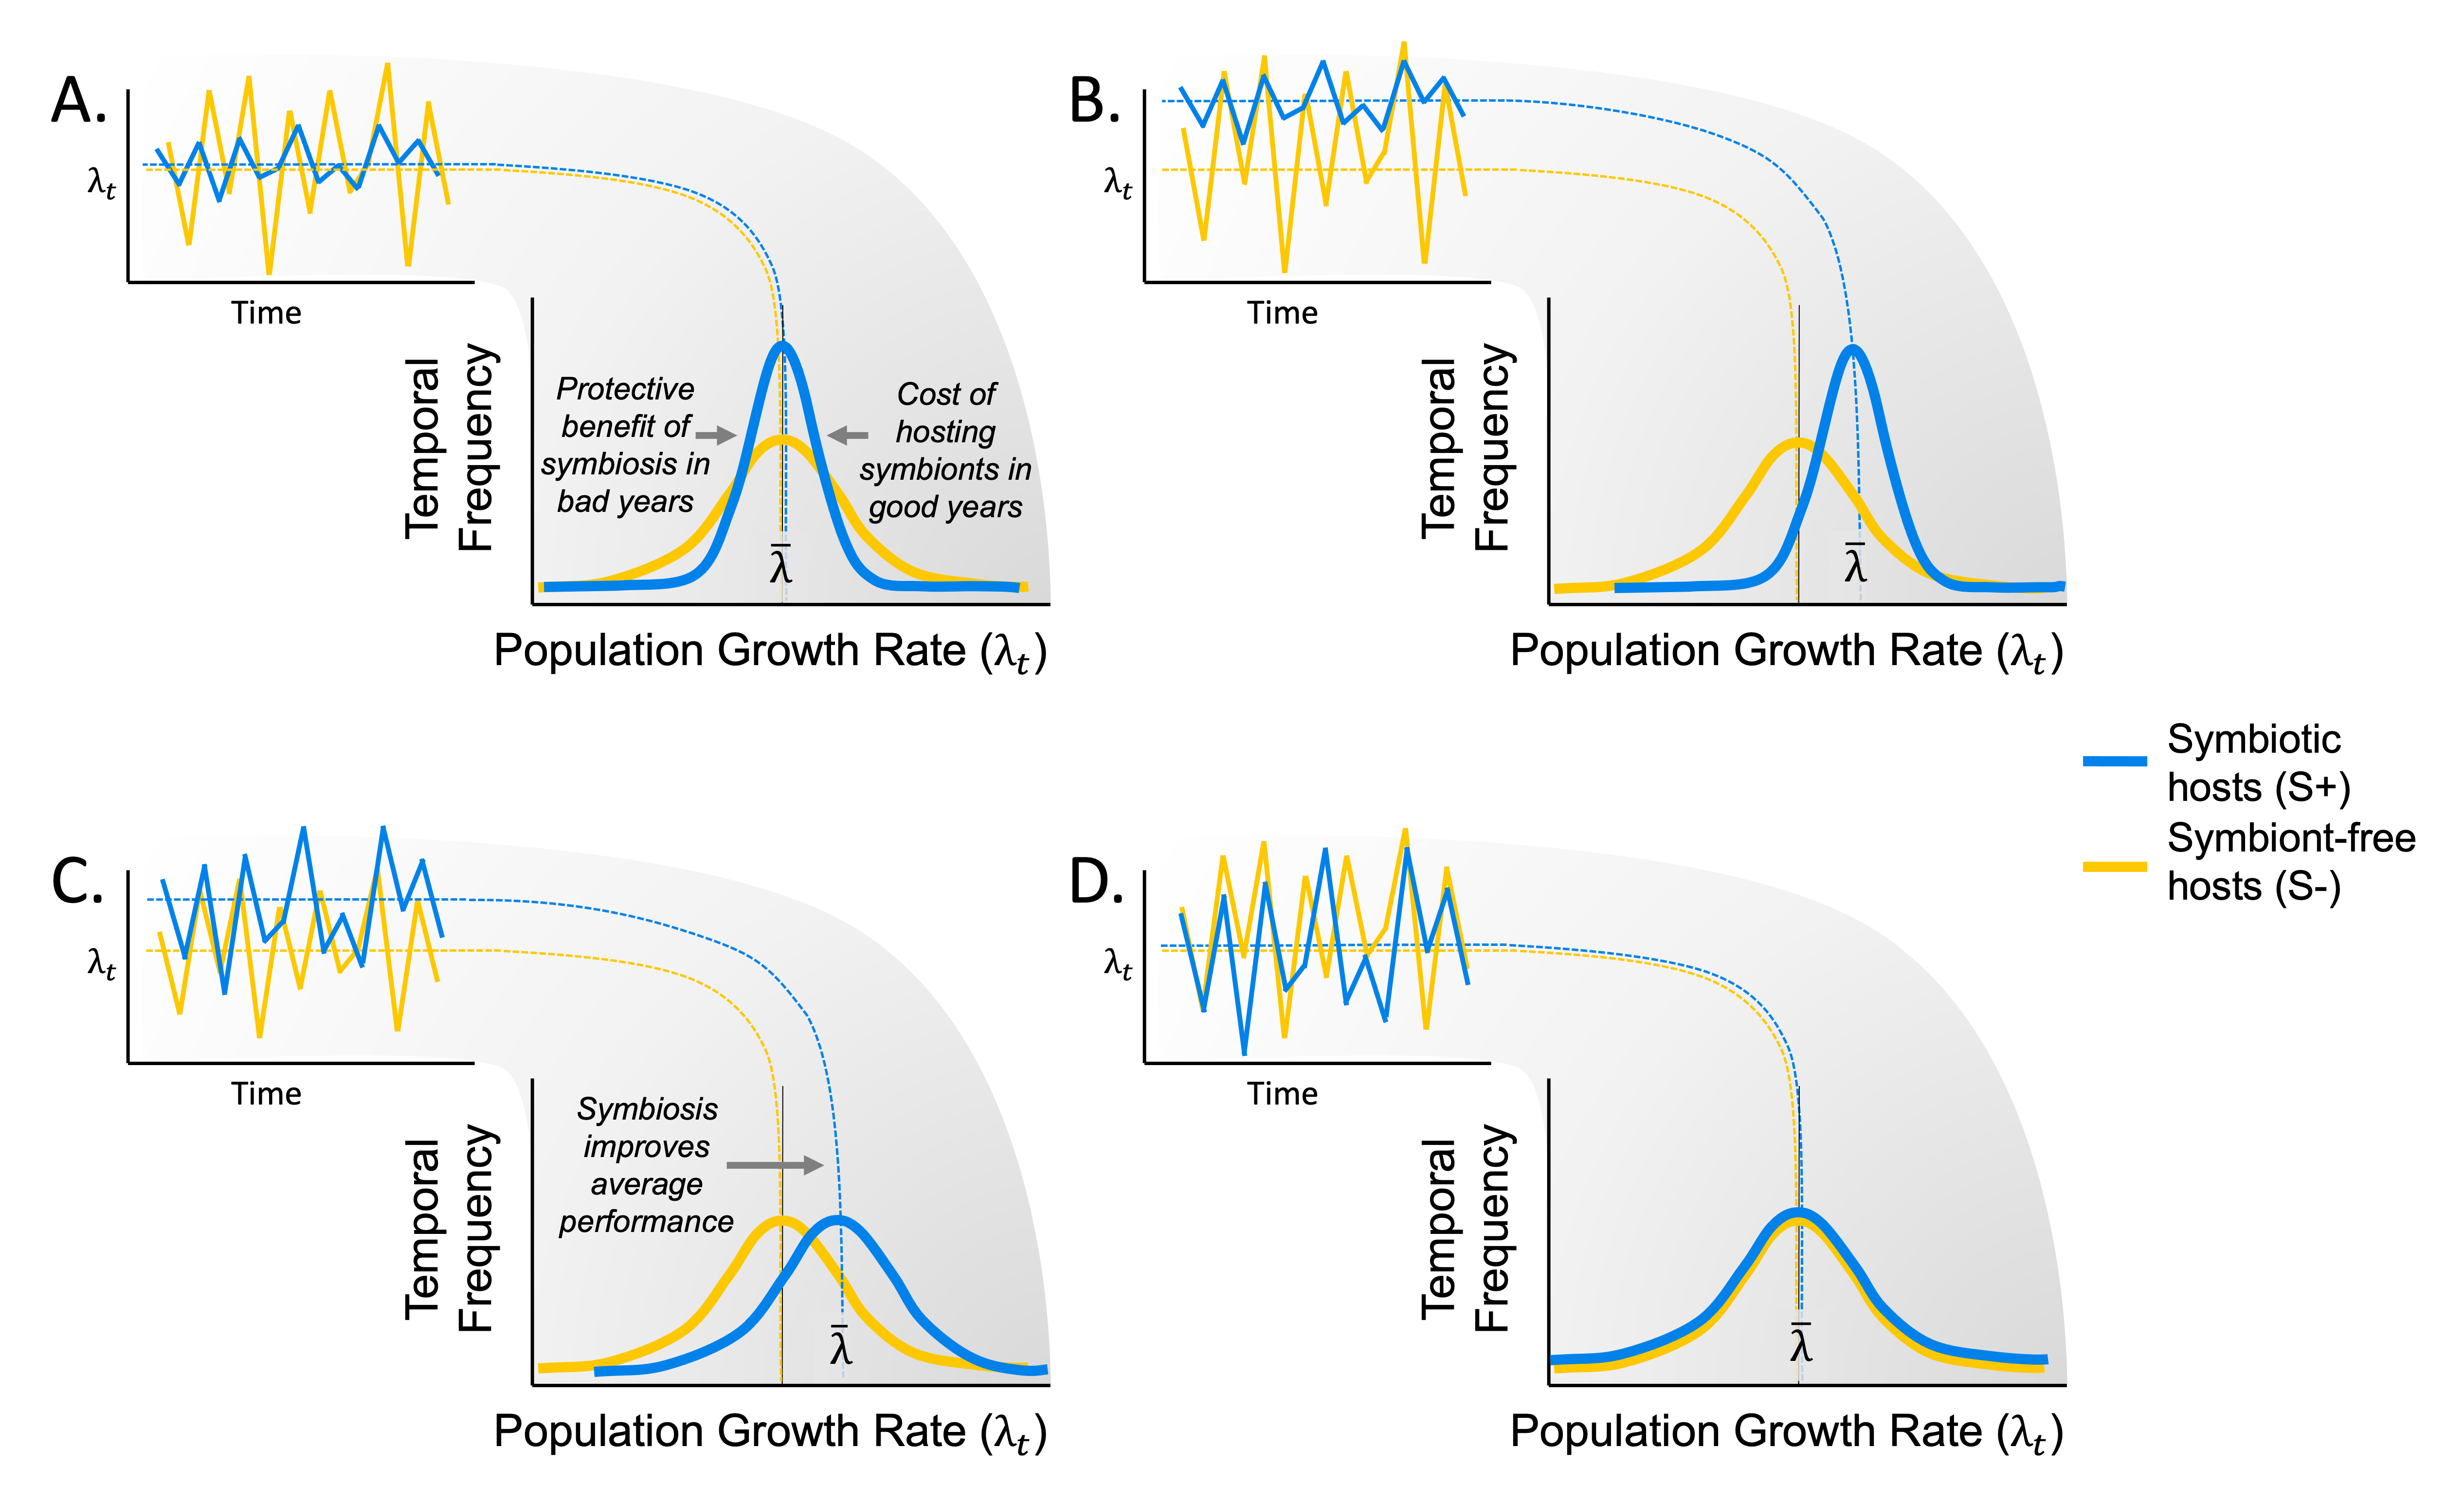
\includegraphics[width=\linewidth]{StochDemo_new_Fig1.png}
	\DIFaddendFL \caption{\DIFdelbeginFL \DIFdelFL{Endophyte }\DIFdelendFL \DIFaddbeginFL \DIFaddFL{Hypothesized effects of }\DIFaddendFL symbiosis \DIFdelbeginFL \DIFdelFL{altered host vital }\DIFdelendFL \DIFaddbeginFL \DIFaddFL{on the mean and variance of annual population growth }\DIFaddendFL rates. (A) \DIFdelbeginFL \DIFdelFL{Shading represents the posterior mean standardized effect size (Cohen's D) of endophyte }\DIFdelendFL \DIFaddbeginFL \DIFaddFL{Context-dependent }\DIFaddendFL symbiosis \DIFdelbeginFL \DIFdelFL{on mean }\DIFdelendFL \DIFaddbeginFL \DIFaddFL{may provide benefits to hosts during harsh years while being neutral }\DIFaddendFL or \DIFdelbeginFL \DIFdelFL{standard deviation }\DIFdelendFL \DIFaddbeginFL \DIFaddFL{costly during benign years.  Temporal variance in populations growth rates }\DIFaddendFL of \DIFaddbeginFL \DIFaddFL{symbiotic }\DIFaddendFL host \DIFdelbeginFL \DIFdelFL{vital rates }\DIFdelendFL \DIFaddbeginFL \DIFaddFL{populations }\DIFaddendFL (\DIFaddbeginFL \DIFaddFL{S+; }\DIFaddendFL blue \DIFdelbeginFL \DIFdelFL{indicates that symbiosis increased the mean or standard deviation and red indicates a reduction}\DIFdelendFL \DIFaddbeginFL \DIFaddFL{lines}\DIFaddendFL ) \DIFaddbeginFL \DIFaddFL{is expected to decrease relative to symbiont-free hosts (S-; yellow lines)}\DIFaddendFL . \DIFdelbeginFL \DIFdelFL{Endophytes' diverse vital rate effects include increased }\DIFdelendFL (B) \DIFdelbeginFL \DIFdelFL{mean growth of }\emph{\DIFdelFL{A. perennans}} %DIFAUXCMD
\DIFdelFL{and }\DIFdelendFL \DIFaddbeginFL \DIFaddFL{Symbiosis may improve average performance across years in addition to reducing temporal variance. }\DIFaddendFL (C) \DIFdelbeginFL \DIFdelFL{mean survival probability }\DIFdelendFL \DIFaddbeginFL \DIFaddFL{Consistent benefits }\DIFaddendFL of \DIFdelbeginFL \emph{\DIFdelFL{F. subverticillata}}%DIFAUXCMD
\DIFdelFL{. Endophyte presence also reduced inter-annual }\DIFdelendFL \DIFaddbeginFL \DIFaddFL{symbiosis could improve average performance across years with no influence on temporal }\DIFaddendFL variance\DIFdelbeginFL \DIFdelFL{in }\DIFdelendFL \DIFaddbeginFL \DIFaddFL{. }\DIFaddendFL (D) \DIFdelbeginFL \DIFdelFL{the survival of }\emph{\DIFdelFL{F. subverticillata}} %DIFAUXCMD
\DIFdelFL{and (E) the fertility of }\emph{\DIFdelFL{P. alsodes}}%DIFAUXCMD
\DIFdelendFL \DIFaddbeginFL \DIFaddFL{Symbiosis may have an effectively neutral effect on population growth rates}\DIFaddendFL .\DIFdelbeginFL \DIFdelFL{In panels B-C, mean vital rate estimates are shown with 80\% credibles along with data binned by size for symbiotic (S+) and symbiont-free (S-) plants, while in panels D-E, annual vital rate estimates are shown along with data binned by size and census year. Organism silhouettes modified from "Festuca subverticillata" by Cindy Roch\'e and "Agrostis hyemalis" and "Poa alsodes" by Sandy Long \copyright Utah State University.}\DIFdelendFL }
\end{figure*}

\DIFaddbegin \begin{figure*}[h]
	\centering
	\includegraphics[width=\linewidth]{StochDemo_fig2new.png}
	\caption{\DIFaddFL{Endophyte symbiosis altered host vital rates.(A) Shading represents the posterior mean standardized effect size (Cohen's D) of endophyte symbiosis on mean or standard deviation of host vital rates (blue indicates that symbiosis increased the mean or standard deviation and red indicates a reduction). Endophytes' diverse vital rate effects include increased (B) mean growth of }\emph{\DIFaddFL{A. perennans}} \DIFaddFL{and (C) mean survival probability of }\emph{\DIFaddFL{F. subverticillata}}\DIFaddFL{. Endophyte presence also reduced inter-annual standard deviation in (D) the survival of }\emph{\DIFaddFL{F. subverticillata}} \DIFaddFL{and (E) the fertility of }\emph{\DIFaddFL{P. alsodes}}\DIFaddFL{. In panels B-C, expected mean vital rates that average across years and plots are shown with 80\% credible intervals along with points representing data binned by size for symbiotic (S+) and symbiont-free (S-) plants. Panels D-E show estimated posterior distributions of endophyte-status specific inter-annual standard deviation ($\sigma^2_{\tau_{e,h}}$)  for each vital rate for S+ (blue) and S- (beige) populations. Organism silhouettes modified from "Festuca subverticillata" by Cindy Roch\'e and "Agrostis hyemalis" and "Poa alsodes" by Sandy Long \copyright Utah State University.}}
\end{figure*}

\DIFaddend \begin{figure*}
	\centering
	\DIFdelbeginFL %DIFDELCMD < 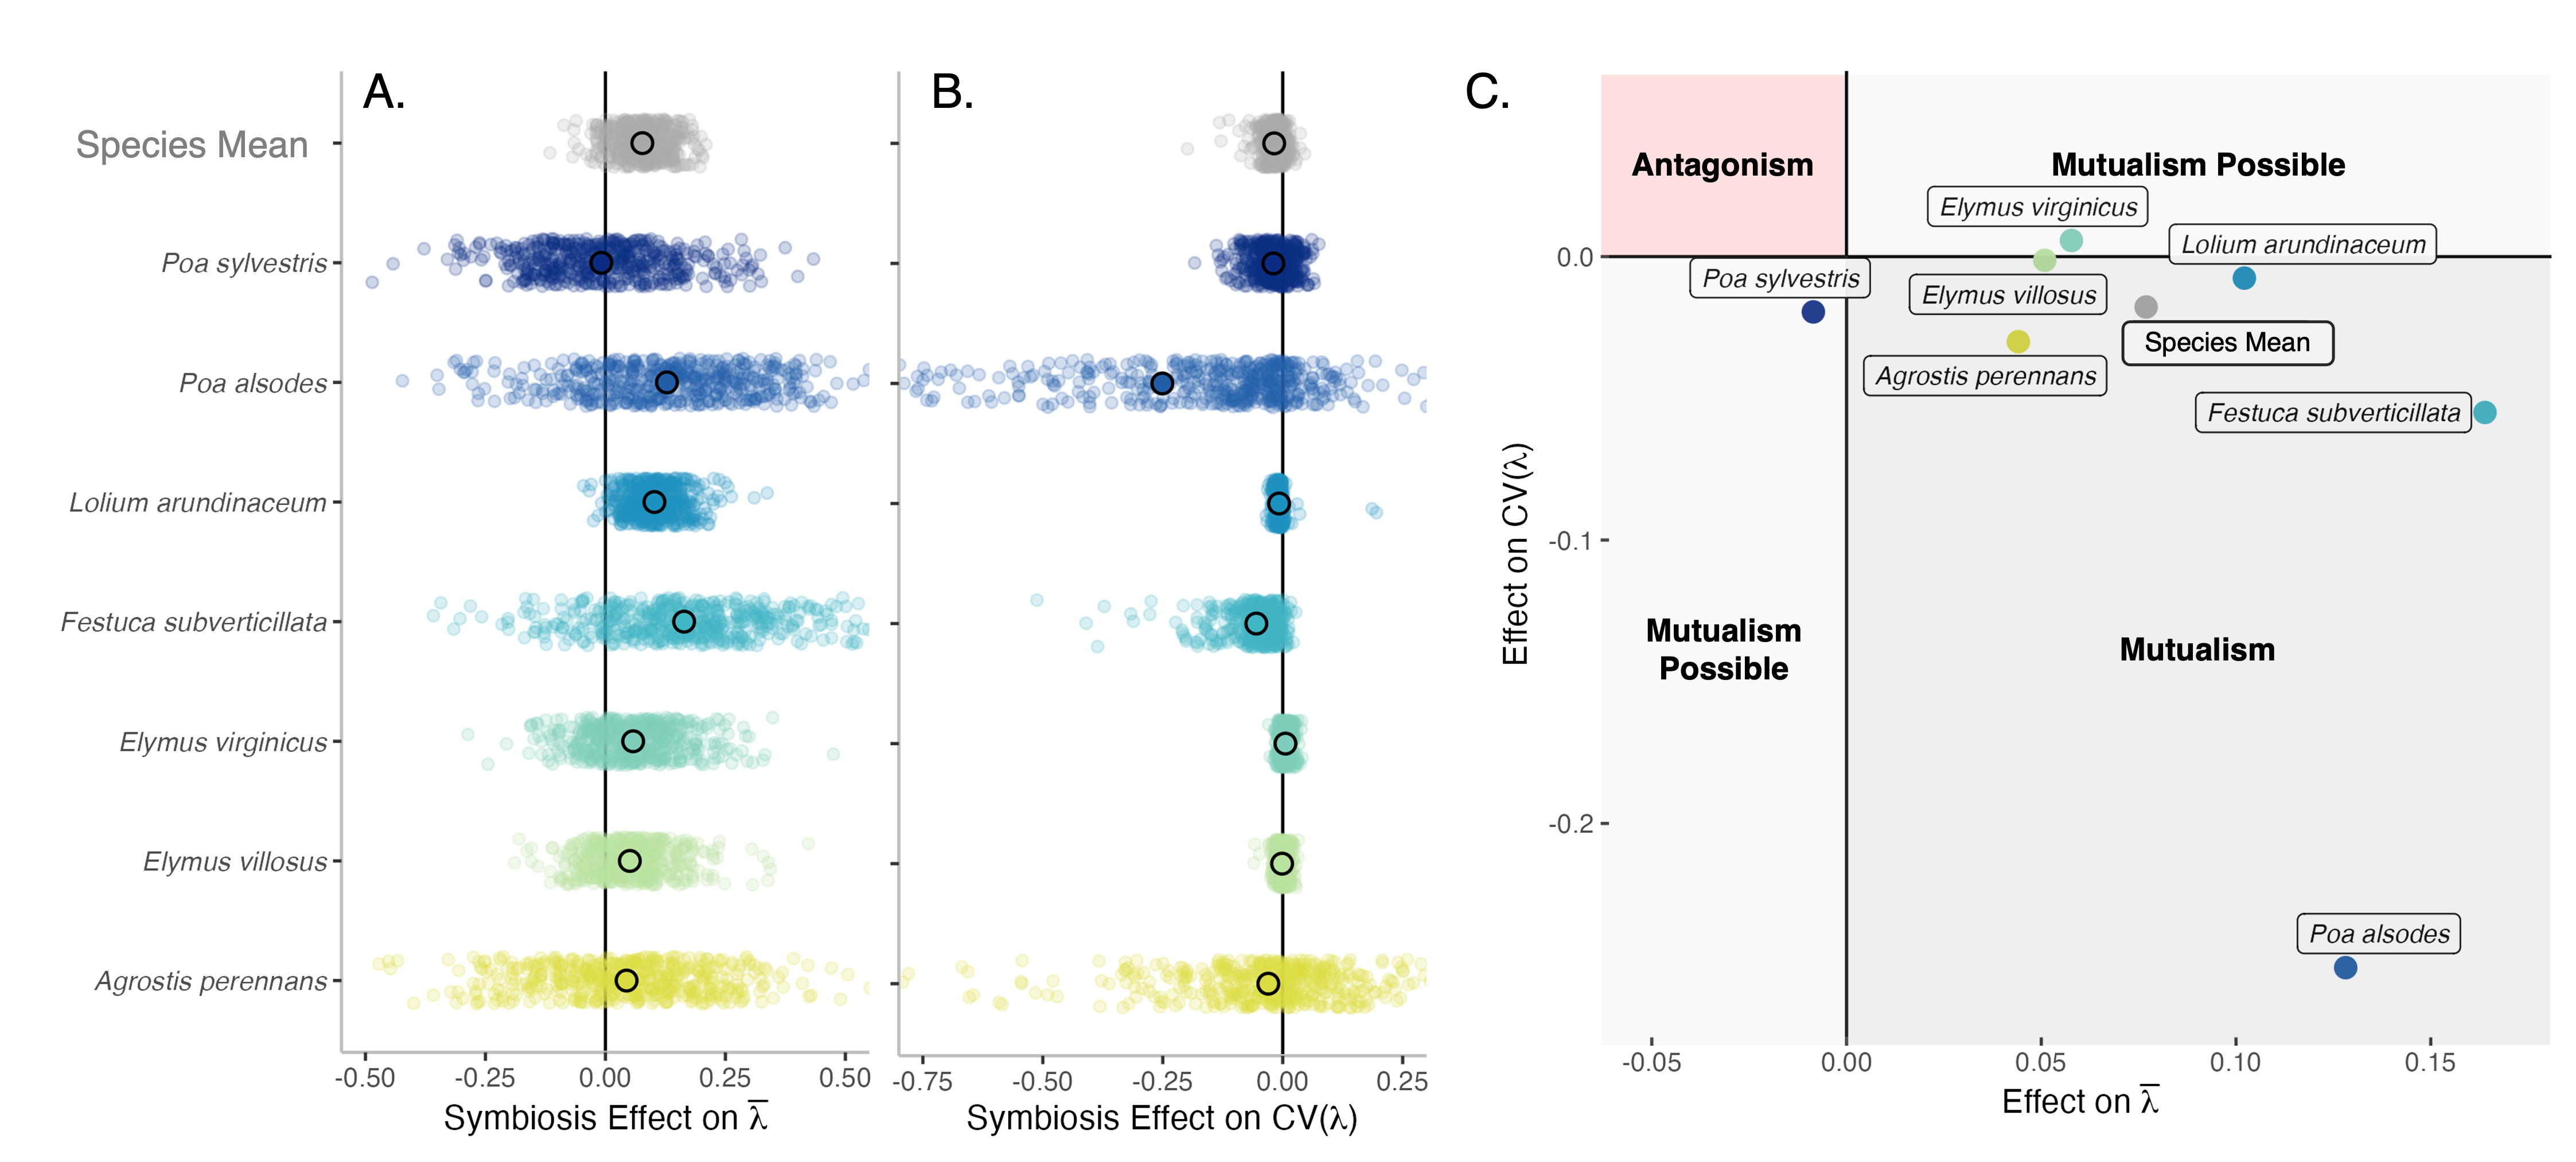
\includegraphics[width =\linewidth]{StochDemo_fig2.png}
%DIFDELCMD < 	%%%
\DIFdelendFL \DIFaddbeginFL 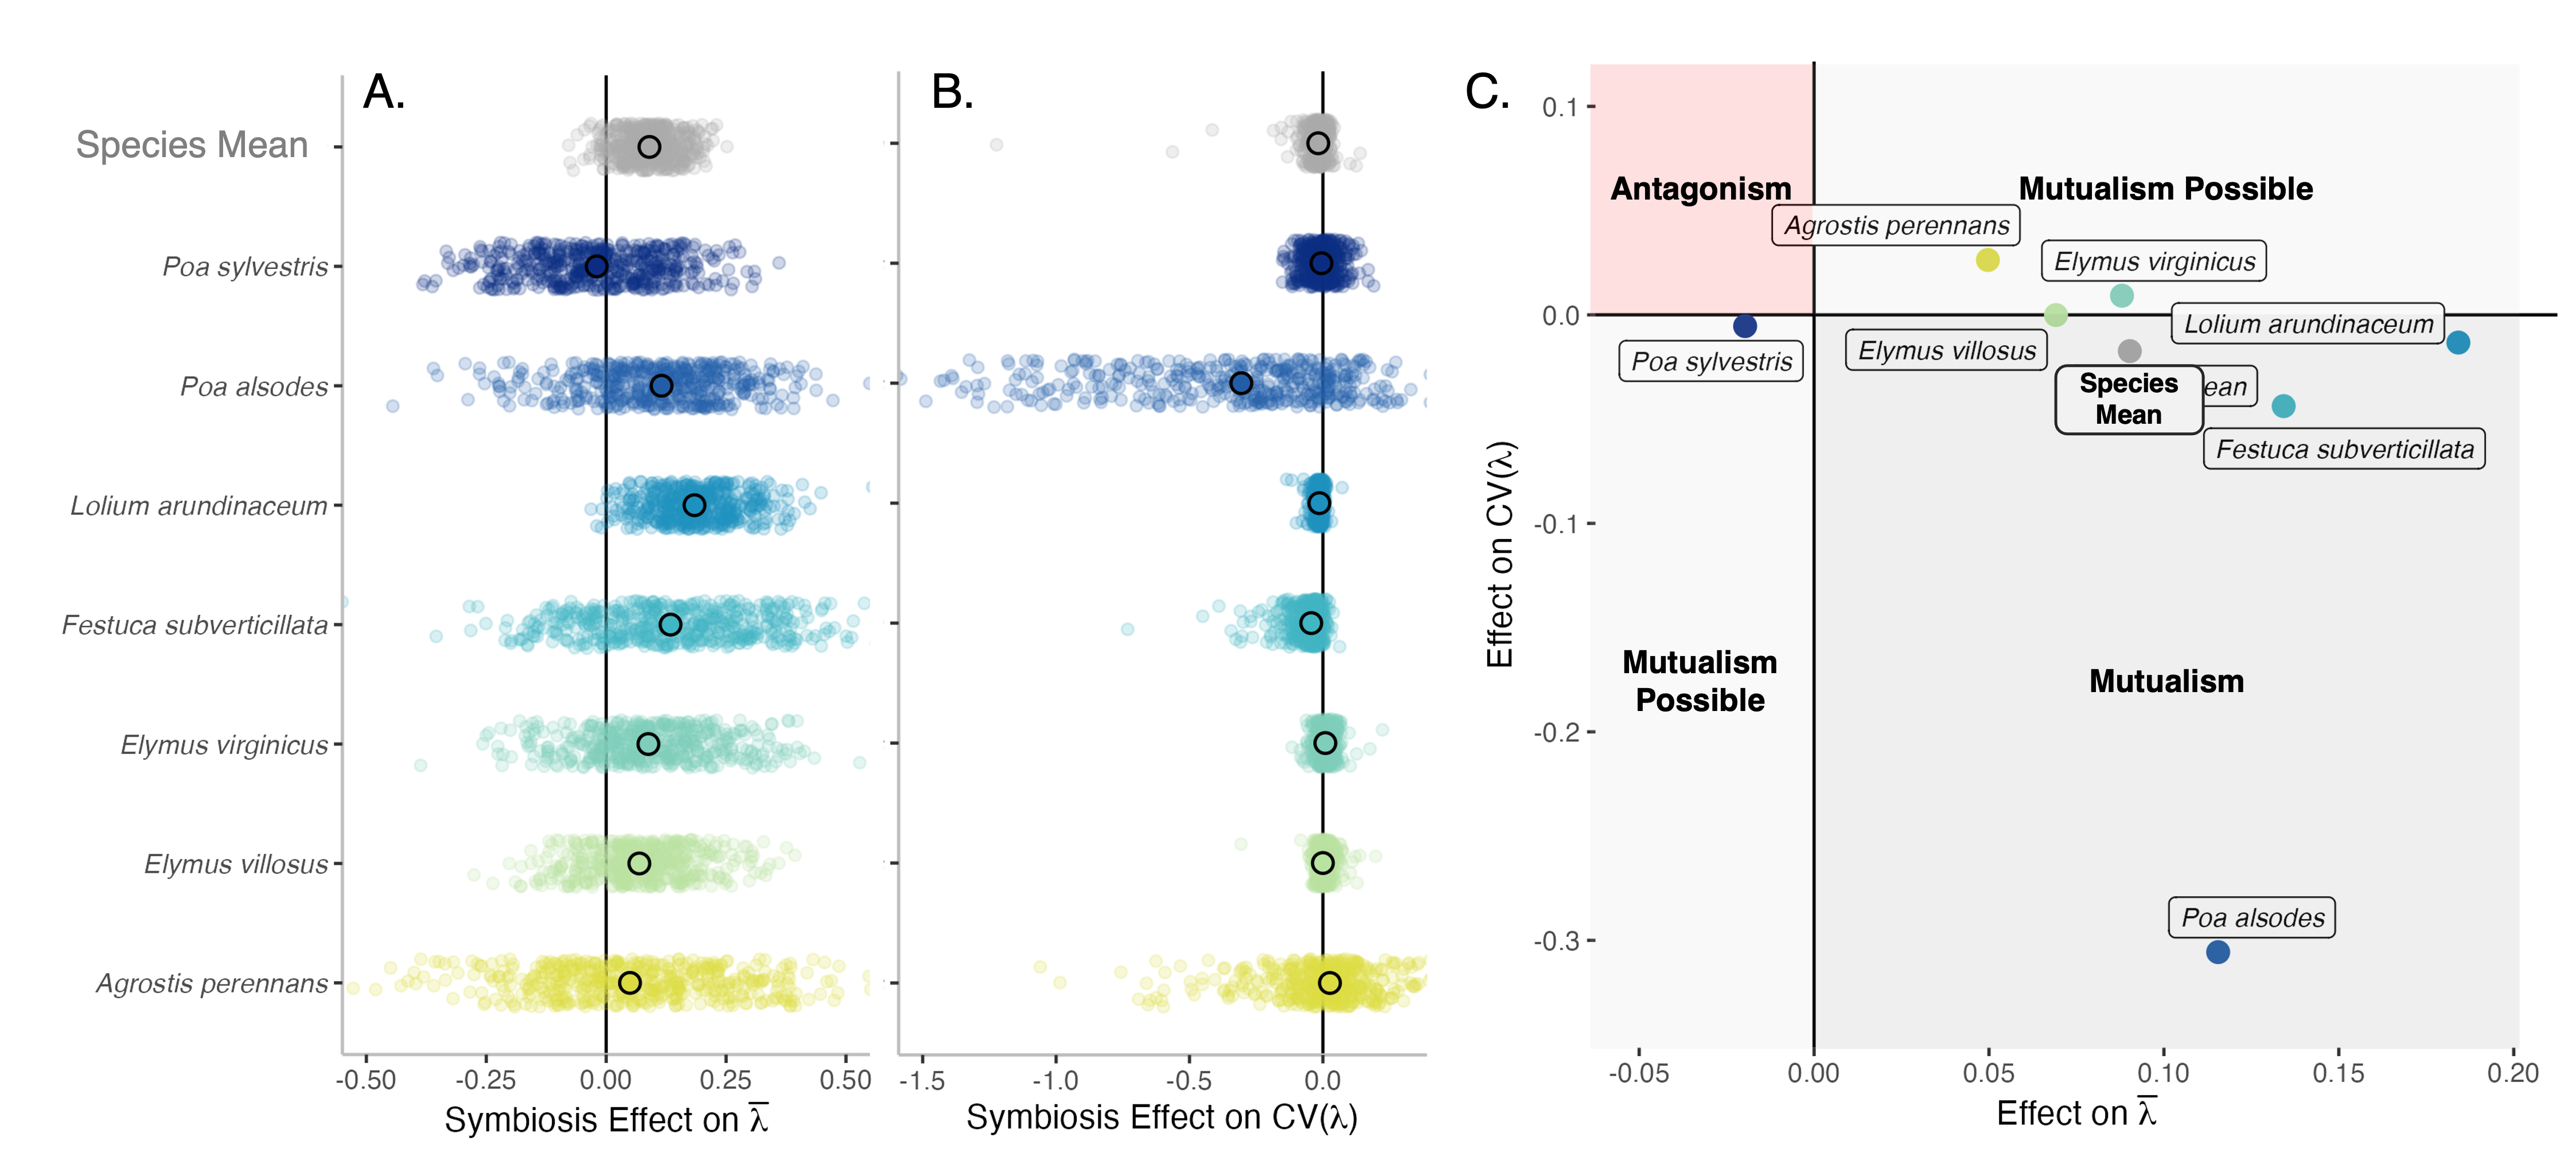
\includegraphics[width =\linewidth]{StochDemo_newFig3.png}
	\DIFaddendFL \caption{Mean and variance-buffering effects on fitness. Black circles indicate the \DIFdelbeginFL \DIFdelFL{average }\DIFdelendFL \DIFaddbeginFL \DIFaddFL{posterior median }\DIFaddendFL effect of endophytes along with 500 posterior draws (smaller colored circles) on the (A) mean and (B) coefficient of variation in \DIFdelbeginFL \DIFdelFL{$\lambda$ }\DIFdelendFL \DIFaddbeginFL \DIFaddFL{$\lambda_{t}$ }\DIFaddendFL for each host species as well as a cross species mean. (C) For all hosts, endophytes either reduce variance, increase the mean, or both, and consequently when considering stochastic environments, the interactions are always at least potentially mutualistic.}
\end{figure*}

\begin{figure*}
	\centering
	\DIFdelbeginFL %DIFDELCMD < 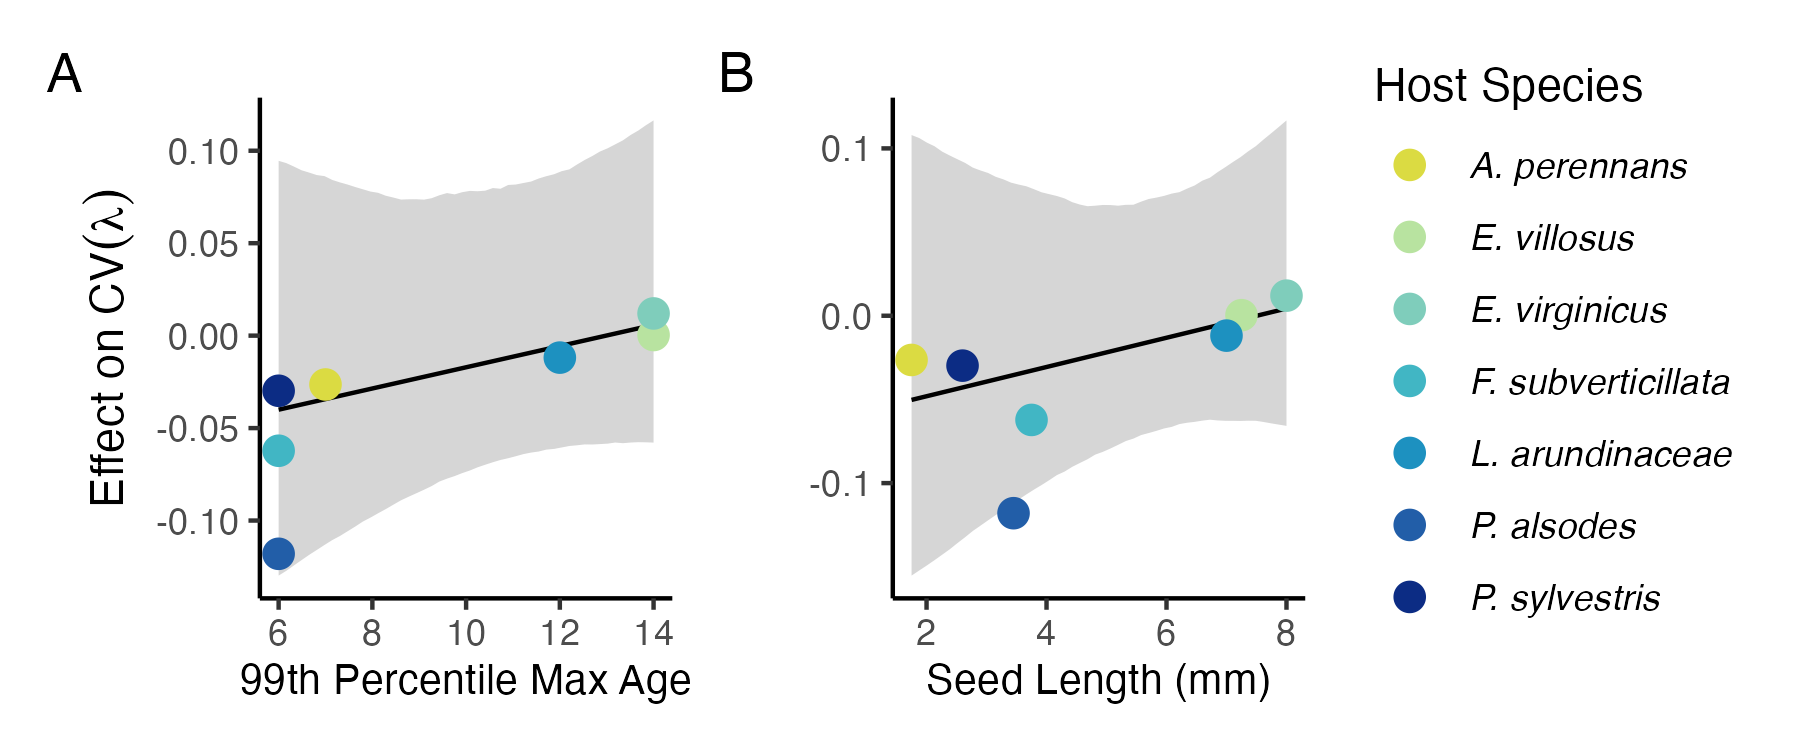
\includegraphics[width=.8\linewidth]{StochDemo_fig3.png}
%DIFDELCMD < 	%%%
\DIFdelendFL \DIFaddbeginFL 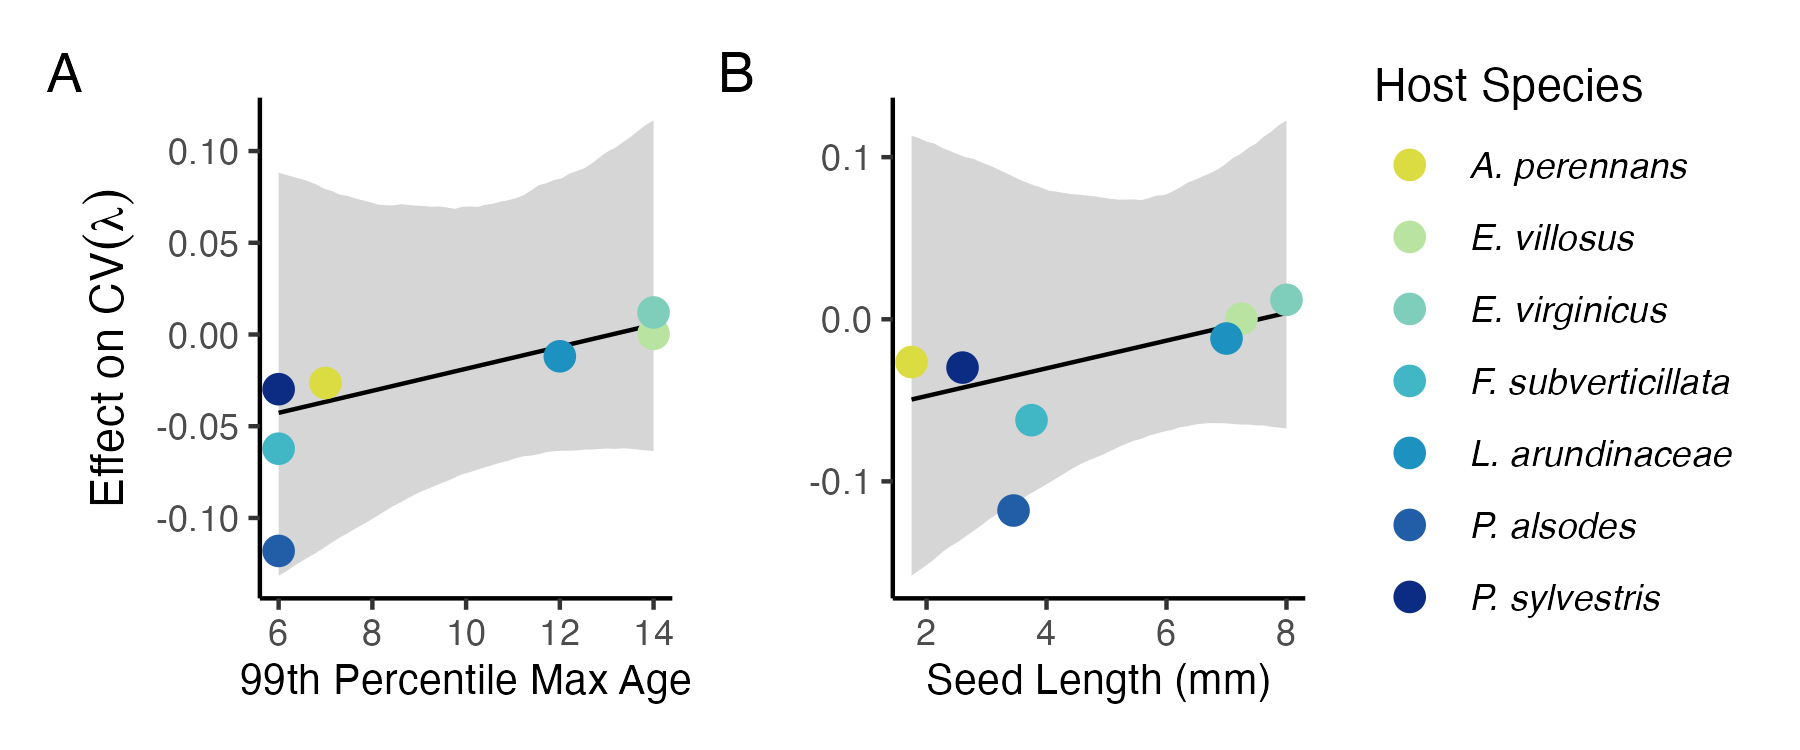
\includegraphics[width=.8\linewidth]{StochDemo_fig4new.png}
	\DIFaddendFL \caption{Host species with faster life history traits experience stronger effects of symbiont-mediated variance buffering. Regressions between life history traits describing the fast-slow life history continuum ((A) 99th percentile maximum age observed during long term censuses in years; (B) Seed size) and the effect of endophyte symbiosis on the coefficent of variation in \DIFaddbeginFL \DIFaddFL{annual }\DIFaddendFL population growth rate (\DIFdelbeginFL \DIFdelFL{$\lambda$}\DIFdelendFL \DIFaddbeginFL \DIFaddFL{$\lambda_{t}$}\DIFaddendFL ). Each panel shows the fitted mean relationship (line) along with the 95\% credible interval.}
\end{figure*}

\begin{figure*}
	\centering
	\DIFdelbeginFL %DIFDELCMD < 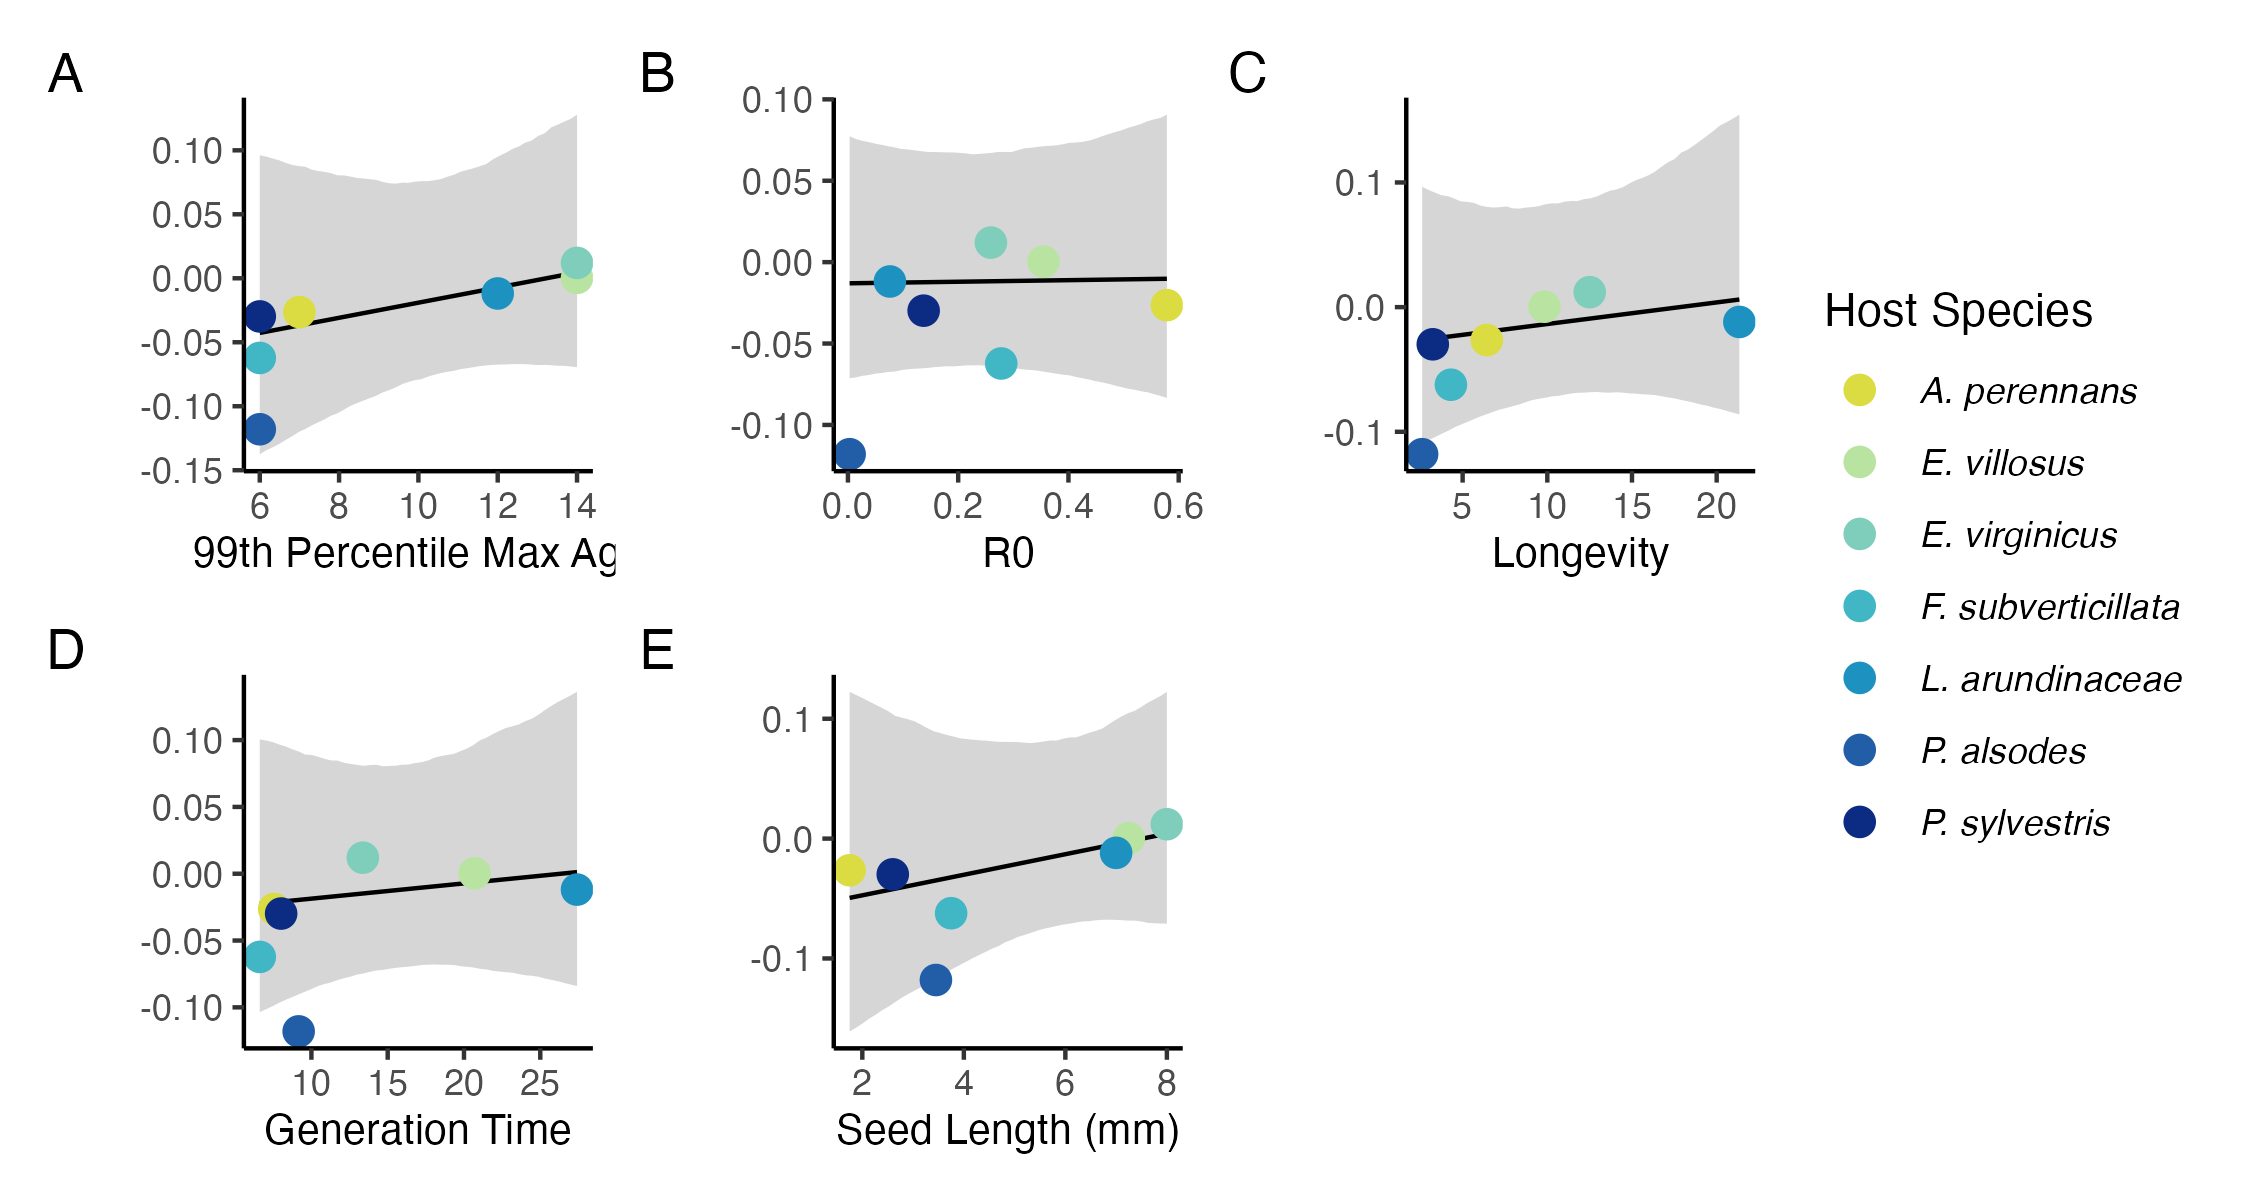
\includegraphics[width=.8\linewidth]{StochDemo_fig4.png}
%DIFDELCMD < 	%%%
\DIFdelendFL \DIFaddbeginFL 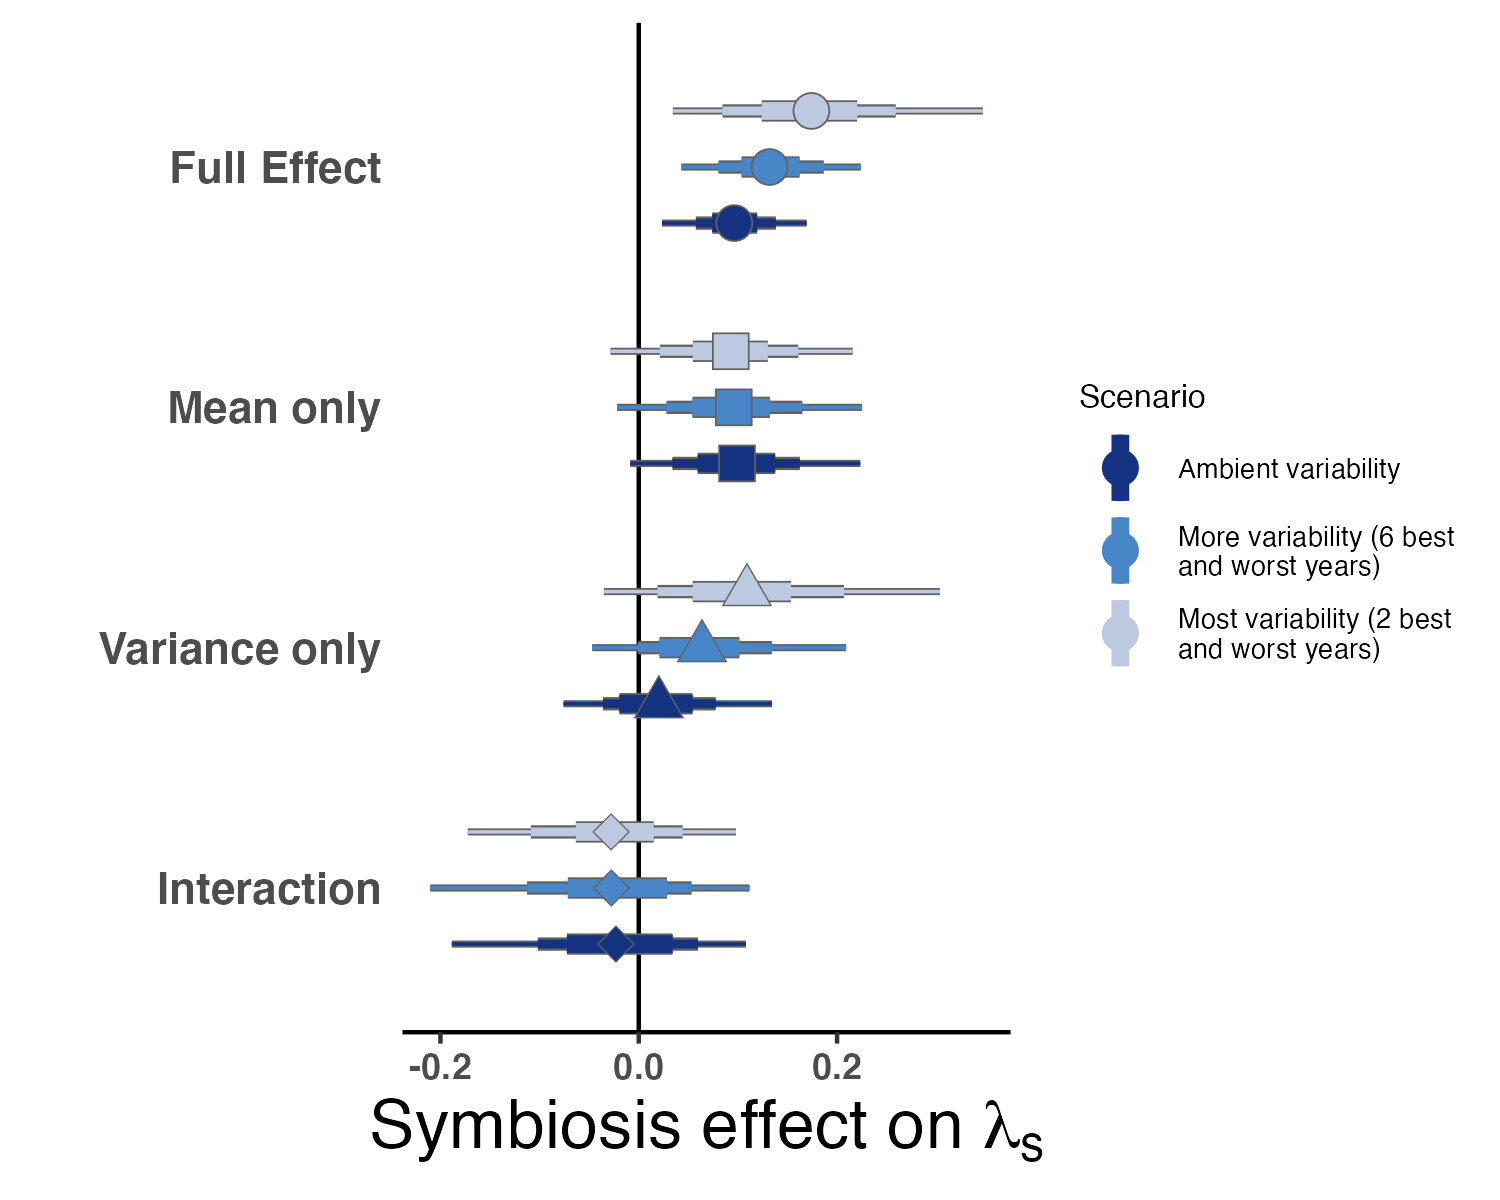
\includegraphics[width=.8\linewidth]{StochDemo_newFig5.png}
	\DIFaddendFL \caption{Cross-species average endophyte contributions to stochastic growth rates under observed and elevated variance. Endophyte symbiosis contributes to the total effect of mutualism on $\lambda_{S}$ through benefits to mean growth rates and through variance buffering as well as the interaction between mean and variance effects. Shapes indicate the posterior mean of each contribution averaged across the seven focal symbiota, along with bars for the 50, 75 and 95\% credible intervals.  The full effect of the symbiosis (circles) becomes more mutualistic under scenarios of increased variance (represented by color shading). Relative to the ambient scenario sampling transition matrices for all 13 transition years during the study period, simulations increased variance by sampling the most extreme six or two years years, leading to increased contributions from variance buffering effects (triangles) and a constant contribution from mean effects (squares).}
\end{figure*}



\clearpage

\begin{appendices}

\section*{Supporting Information}\label{secA}

\DIFdelbegin \subsubsection*{\DIFdel{Supplemental Methods}}

%DIFAUXCMD
\DIFdelend \DIFaddbegin \subsection*{\DIFadd{Supplemental Methods}}
\renewcommand\theequation{S\arabic{equation}}   

\DIFaddend 

	\DIFdelbegin \subsubsection*{\DIFdel{Estimating climate drivers of environmental context-dependence}}%DIFAUXCMD
%DIFDELCMD < {
%DIFDELCMD < 

%DIFDELCMD < 	%%%
\DIFdel{To connect the variance buffering effects of endophytes with inter-annual variability in climate}\DIFdelend \DIFaddbegin \subsubsection*{\DIFadd{Endophyte removal}\DIFaddend , \DIFdelbegin \DIFdel{we built climate-explicit stochastic matrix population models from the vital rate data in addition to the climate-implicit model described in the main text. 
	Identifying the potentially complex relationships between vital rates and environmental drivers remains a key challenge for accurate forecasts of the ecological impacts of environmental stochasticity \mbox{%DIFAUXCMD
\cite{ehrlen2015predicting}}\hspace{0pt}%DIFAUXCMD
.
	We first downloaded temperature and precipitation data from a weather station in Bloomington}\DIFdelend \DIFaddbegin \DIFadd{plant propagation}\DIFaddend , \DIFdelbegin \DIFdel{IN,  approx. 27 km from our study site, using the rnoaa package \mbox{%DIFAUXCMD
\cite{chamberlain2022package}}\hspace{0pt}%DIFAUXCMD
. 
	Compared to other weather stations in the area, the measurements from Bloomington contain the most complete climate record across the study period }\DIFdelend and \DIFdelbegin \DIFdel{are correlated with more local measurements }\DIFdelend \DIFaddbegin \DIFadd{field set-up}}
\DIFadd{Seeds from naturally symbiotic populations of the seven focal host species were collected during summer-fall 2006 }\DIFaddend from \DIFdelbegin \DIFdel{Nashville}\DIFdelend \DIFaddbegin \DIFadd{Lilly-Dickey Woods and the nearby Bayles Road Teaching and Research Preserve (39.220167}\DIFaddend , \DIFdelbegin \DIFdel{IN for years in which local data are available }\DIFdelend \DIFaddbegin \DIFadd{-86.542683). 
To generate symbiotic (S+) and symbiont-free }\DIFaddend (\DIFdelbegin \DIFdel{total daily precipitation: $R^2$ = .76; mean daily temperature: $R^2$ = .94).
	The mean annual temperature across the study period was 11.9 $C^o $ (SD: 1.05 $C^o $) and the average annual precipitation was 1237.9 mm/year (SD: 204.89 mm/year) (Fig. S24).
	Given the known role of endophytes in promoting host drought tolerance, we calculated the Standardised Precipitation-Evapotranspiration Index (SPEI) for 3 and 12 months preceding each annual censuses, reflecting drought during the growing season and across the year \mbox{%DIFAUXCMD
\cite{vicente2010multiscalar}}\hspace{0pt}%DIFAUXCMD
.
	To calculate SPEI, we used the Thornthwaite equation to model potential evapotranspiration as implemented in the SPEI R package \mbox{%DIFAUXCMD
\cite{begueria2013spei}
	
}\hspace{0pt}%DIFAUXCMD
}\DIFdelend \DIFaddbegin \DIFadd{S-) plants from the same genetic lineages, seeds from each species were disinfected with a heat treatment described in Table S1 or left untreated. 
The heat treatment created symbiont-free plants by warming seeds to temperatures at which the fungus becomes inviable but the host seeds can still germinate.

}\DIFaddend 


\DIFdelbegin \DIFdel{We repeated the process of fitting statistical models for each vital rate as described in }\textbf{\DIFdel{Materials and Methods}} %DIFAUXCMD
\DIFdel{with the inclusion of a parameter describing the influence of SPEI. 
	We fit separate vital rate models incorporating either the growing season or annual drought index for each vital rate}\DIFdelend \DIFaddbegin \DIFadd{Both heat-treated and untreated seeds were surface sterilized with bleach to remove epiphyllous microbes, cold stratified for up to 4 weeks, then germinated in a growth chamber before transfer to the greenhouse at Indiana University where they grew for $\sim$ 8 weeks. 
We confirmed endophyte status by staining thin sections of inner leaf sheath with aniline blue and examining tissue for fungal hyphae at 200X magnification \mbox{%DIFAUXCMD
\cite{bacon2018stains}}\hspace{0pt}%DIFAUXCMD
. 
We established experimental populations with vegetatively propagated clones of similar sizes (ranging from one to six tillers). 

}

\DIFadd{During the fall of 2007 and spring of 2008, we established 10 3x3 m plots for }\emph{\DIFadd{A. perennans}}\DIFaddend , \DIFdelbegin \DIFdel{except for the model describing the mean number of seeds per inflorescence. 
	This model was fit without climate effects because the data came from only a few years.
	Initial analyses indicated similar fits for models including only a linear term and those with both linear and quadratic terms describing the relationship between the climate driver and the vital rate response}\DIFdelend \DIFaddbegin \emph{\DIFadd{E. villosus}}\DIFaddend , \DIFdelbegin \DIFdel{and so we proceeded with models including only the linear term.
	We expected that including climate predictors into the models would explain some inter-annual variance in vital rates}\DIFdelend \DIFaddbegin \emph{\DIFadd{E. virginicus}}\DIFaddend , \DIFdelbegin \DIFdel{shrinking the variance associated with the fitted year random effects.
	We assessed model fit with graphic posterior predictive checks }\DIFdelend \DIFaddbegin \emph{\DIFadd{F. subverticillata}}\DIFadd{, and }\emph{\DIFadd{L. arundinaceum}}  \DIFaddend and \DIFdelbegin \DIFdel{convergence diagnostics as described for the climate-implicit analysis. 
	Finally, we next built matrix projection models incorporating the climate-dependent vital rate functions to assess the response of symbiotic (S}\DIFdelend \DIFaddbegin \DIFadd{18 plots for }\emph{\DIFadd{P. alsodes}} \DIFadd{and }\emph{\DIFadd{P. sylvestris}}\DIFadd{.
Half of the plots were randomly assigned to be planted with either symbiotic (S}\DIFaddend +\DIFdelbegin \DIFdel{) vs }\DIFdelend \DIFaddbegin \DIFadd{) or }\DIFaddend symbiont-free (S-\DIFdelbegin \DIFdel{) populations to drought. 
	The model is as described in }\textbf{\DIFdel{Materials and Methods}} %DIFAUXCMD
\DIFdel{with the inclusion of parameters describing the slope of the relationship with SPEI. 
	We compared the sensitivity of $\lambda$ to either annual or seasonal SPEI of S}\DIFdelend \DIFaddbegin \DIFadd{) plants, and initiated with 20 evenly spaced individuals labeled with aluminum tags.
In spring 2008, we placed plastic deer net fencing around each plot to limit deer herbivory and disturbance; damaged fences were regularly replaced.

}


\DIFadd{We expected plots to maintain their endophyte status (S}\DIFaddend + \DIFdelbegin \DIFdel{populations ($\frac{\Delta\lambda^{+}}{\Delta SPEI}$) with those of }\DIFdelend \DIFaddbegin \DIFadd{or }\DIFaddend S-\DIFdelbegin \DIFdel{populations ($\frac{\Delta\lambda^{-}}{\Delta SPEI}$)(Fig. S25; Table S).
	
}%DIFDELCMD < 

%DIFDELCMD < 	%%%
\DIFdel{Most species were slightly more responsive to growing season rather than annual drought conditions}\DIFdelend \DIFaddbegin \DIFadd{) because these fungal symbionts are almost exclusively vertically transmitted, and plots were spaced a minimum of 5 m apart, limiting seed dispersal or horizontal transmission of the symbiont between plots. 
We regularly confirmed endophyte treatment throughout the lifetime of the experiment by opportunistically taking subsets of seeds from reproductive individuals and scoring them for their endophyte status with microscopy as above.
Overall, these scores reflected 98\% faithfulness of recruits to their expected endophyte status across species and plots (Fig. S87; Supplement data). 
Additionally, we have rarely observed fungal stromata, the fruiting bodies by which }\emph{\DIFadd{Epichlo\"e}} \DIFadd{are potentially transmitted horizontally, provided the fly vector is also present \mbox{%DIFAUXCMD
\cite{bultman1995mutualistic}}\hspace{0pt}%DIFAUXCMD
. 
For }\emph{\DIFadd{A. perennans}}\DIFaddend , \DIFaddbegin \emph{\DIFadd{F. subverticillata}}\DIFadd{, }\emph{\DIFadd{L. arundinaceum}}\DIFadd{, and }\emph{\DIFadd{P. alsodes}}\DIFadd{, we never observed stromata. 
We observed stromata only infrequently for }\emph{\DIFadd{E. villosus}}\DIFadd{, and even more rarely for }\emph{\DIFadd{E. virginicus}} \DIFaddend and \DIFdelbegin \DIFdel{for most species symbiotic populations were less sensitive to SPEI than symbiont-free populations (Fig. S25; Table S3).
	However}\DIFdelend \DIFaddbegin \emph{\DIFadd{P. sylvestris}} \DIFadd{(Table S2). 
For these species, stromata have only been observed irregularly across years on 35}\DIFaddend , \DIFdelbegin \DIFdel{these drought indices did not explain the full extent of inter-annual variability in demographic vital rates.
	For example, flowering in }\emph{\DIFdel{A. perennans}} %DIFAUXCMD
\DIFdel{had one of the strongest climate signals }\DIFdelend \DIFaddbegin \DIFadd{4, and 6 plants respectively, making up $< 0.3$\% of all censused plants.

}

\subsubsection*{\DIFadd{Detailed vital rate modeling}}

\DIFadd{We fit vital rates models in a Bayesian hierarchical framework. 
Statistical models for adult survival, seedling survival, adult growth, seedling growth, flowering (yes or no), fertility of flowering plants (number of flowering tillers), production of seed-bearing spikelets (number per inflorescence), the average number of seeds per spikelet, and the recruitment of seedlings from the preceding year's seed production, were constructed as follows:

}

\emph{\DIFadd{Survival}} \DIFadd{- We modeled survival as a Bernoulli process, where the survival ($S$) of an individual $i$ in plot $p$ and census year $t$ was predicted by the plot-level endophyte status ($e$), host species ($h$), size in the preceding census, and the plant's origin status ($o$; whether it was initially transplanted or naturally recruited into the plot).

}

\begin{subequations}
	\label{eq:survival}
	\begin{align}
		S_{i,p,e,h,t} \sim Bernoulli(\hat{S}_{i,p,e,h,t})\\
		logit(\hat{S}_{i,p,e,h,t}) = \beta_{0_{h,o}} + \beta_{1_{h}}*endo_{e}\\
		 + \beta_{2_{h,o}}*size_{i,t-1} +\beta_{3_{h,o}}*size^2_{i,t-1} + \tau_{e,h,t} + \rho_{p}\\
		\tau_{e,h,t} \sim Normal(0,\sigma^2_{\tau_{e,h}})\\
		\rho_{p} \sim Normal(0,\sigma^2_{\rho})
	\end{align}
\end{subequations}

\DIFadd{Here, $\hat{S}$ is the survival probability, $\beta_{0_{h,o}}$ is an intercept specific to each host species and recruitment origin, $\beta_{1_{h}}$ is the endophyte effect, $\beta_{2_{h,o}}$ is the effect of plant size specific to each species and recruitment origin, $\beta_{3_{h,o}}$ is a quadratic plant size effect specific to each species and recruitment origin, $\tau_{e,h,t}$ is a normally distributed year effect for each species and endophyte status with variance $\sigma^2_{\tau_{e,h}}$, and $\rho_{p}$ is a normally distributed plot effect with variance $\sigma^2_{\rho}$ }\DIFaddend (\DIFdelbegin \DIFdel{$82\%$ probability of a positive relationship with SPEI), yet the estimated inter-annual }\DIFdelend \DIFaddbegin \DIFadd{$p(e)$ indicates that plot identity is uniquely associated with an endophyte status).
We assume that the plot-to-plot }\DIFaddend variance \DIFdelbegin \DIFdel{$\sigma^2_{\tau_{P}}$ for symbiont-free plants shrank from 6.7 to 6.1 after including 3-month SPEI as a covariate, suggesting that other factors contribute to }\DIFdelend \DIFaddbegin \DIFadd{$\sigma^2_{\rho}$ was shared across host species, allowing us to ``borrow strength'' across the multi-species dataset; other model parameters are unique to host species. 
We separately modeled the survival of newly recruited seedlings with a similar model but omitting previous size dependence and origin status. 
%DIF > All random effects were estimated independently between seedling and adult vital rates models.

}


\emph{\DIFadd{Growth}} \DIFadd{- We modeled plant size in census year $t$ ($G$) with the same linear predictor for the mean as described for survival.
Because we measured size as positive integer-valued counts of tillers, we modeled it with a zero-truncated Poisson-inverse Gaussian distribution.
This distribution includes a shape parameter $\lambda_G$ to account for overdispersion in the data.
We additionally modeled the growth of newly recruited seedlings separately with a Poisson-inverse Gaussian model omitting size structure and the plants' origin status as with seedling survival.

}

\emph{\DIFadd{Flowering}} \DIFadd{- We modeled whether or not a plant was flowering during the census ($P$) as a Bernoulli process, with the same linear predictor for the mean as described above for survival except that size dependence for reproductive vital rates was determined by the individual's size during the same census year as opposed to its size during the previous year.

}

\emph{\DIFadd{Fertility}} \DIFadd{- For a plant that was flowering during the census, its fertility was the number of reproductive tillers produced ($F$), which we modeled as a function of size in the same census period with a zero-truncated Poisson-Inverse Gaussian distribution, with the same linear predictor for the mean as described above. 

}

\emph{\DIFadd{Spikelets per Inflorescence}} \DIFadd{- Spikelet production ($K$) was recorded as integer counts on up to three inflorescences per reproducing plant.
We modeled these data with a negative binomial distribution, with the same linear predictor for the mean as described above. 

}

\emph{\DIFadd{Seed Production per Spikelet}} \DIFadd{- For individuals with recorded counts of seed production, we calculated the number of seeds per spikelet from our counts of seeds and spikelets per inflorescence, and then modeled seeds per spikelet ($D$) as means of a Gaussian distribution for each species and endophyte status. 
Because we had less detailed data across years and plants for seed production than for other reproductive vital rates, we omitted both plot and year random effects. 

}

\emph{\DIFadd{Seedling Recruitment}} \DIFadd{- We used a binomial distribution to model the recruitment of new seedlings ($R$) into the plots from seeds produced in the preceding year, assuming no long-lived seed bank. 
We included an intercept specific to each host and endophyte status and the same random effects structure as in other models. 
We estimated the number of seeds per plot in the preceding year by multiplying the total number of reproductive tillers per plant by the mean number of spikelets per inflorescence and mean number of seeds per spikelet ($D$).
For plants with missing fertility or spikelet data, we used the expected number of reproductive tillers ($F$) or of spikelets per inflorescence from ($K$), drawing from the full posteriors of our models. 
We rounded this value to get the estimated seed production for each individual, and finally summed across all reproductive plants in each year and plot to get the total number of seeds produced. 

}

\textbf{\DIFadd{Model assessment}}\\
\DIFadd{All parameters were given vague priors \mbox{%DIFAUXCMD
\cite{gabry2019visualization}}\hspace{0pt}%DIFAUXCMD
.
We ran each vital rate model for 2500 warm-up and 2500 MCMC sampling iterations with three chains. 
We assessed model convergence with trace plots of posterior chains and checked for $\hat{R}$ values less than 1.01, indicating low within- and between-chain variation \mbox{%DIFAUXCMD
\cite{brooks1998general,gelman2006data}}\hspace{0pt}%DIFAUXCMD
. 
For those models that showed poor convergence, we extended the MCMC sampling to include 5000 warm-up and 5000 sampling iterations, which was only necessary for seedling growth.
We visualized the interactions between plant size, origin status, and endophyte status for both the interannual mean expected value for each vital rate (averaging over year and plot variance) (Fig. S2 - S11) and for the expected vital rate values specific to each year (averaging over plot variance) (Fig. S12 -S21).
We graphically checked vital rate model fit with posterior predictive checks comparing simulated and observed data (Fig. S30-S68).
Initial analyses including only linear effects of size produced estimates of endophytes' effects on vital rate means and }\DIFaddend inter-annual \DIFdelbegin \DIFdel{variability.
}%DIFDELCMD < }
%DIFDELCMD < %%%
\DIFdelend \DIFaddbegin \DIFadd{variances that were similar to those from the more flexible quadratic models, but provided worse fit to size-structure in the data in some cases. 
We therefore proceeded with the more flexible quadratic models. 
Results from subsequent matrix model analyses were qualitatively similar regardless of this choice.

}


\subsubsection*{Estimating climate drivers of environmental context-dependence}{

	\DIFadd{To connect the variance buffering effects of endophytes with inter-annual variability in climate, we built climate-explicit stochastic matrix population models from the vital rate data in addition to the climate-implicit model described in the main text. 
	Identifying the potentially complex relationships between vital rates and environmental drivers remains a key challenge for accurate forecasts of the ecological impacts of environmental stochasticity \mbox{%DIFAUXCMD
\cite{ehrlen2015predicting}}\hspace{0pt}%DIFAUXCMD
.
	We first downloaded temperature and precipitation data from a weather station in Bloomington, IN,  approx. 27 km from our study site, using the rnoaa package \mbox{%DIFAUXCMD
\cite{chamberlain2022package}}\hspace{0pt}%DIFAUXCMD
. 
	Compared to other weather stations in the area, the measurements from Bloomington contain the most complete climate record across the study period and are correlated with more local measurements from Nashville, IN for years in which local data are available (total daily precipitation: $R^2$ = .76; mean daily temperature: $R^2$ = .94).
	The mean annual temperature across the study period was 11.9 $C^o $ (SD: 1.05 $C^o $) and the average annual precipitation was 1237.9 mm/year (SD: 204.89 mm/year) (Fig. S88).
	Given the known role of endophytes in promoting host drought tolerance, we calculated the Standardised Precipitation-Evapotranspiration Index (SPEI) for 3 and 12 months preceding each annual censuses, reflecting drought during the growing season and across the year \mbox{%DIFAUXCMD
\cite{vicente2010multiscalar}}\hspace{0pt}%DIFAUXCMD
.
	To calculate SPEI, we used the Thornthwaite equation to model potential evapotranspiration as implemented in the SPEI R package \mbox{%DIFAUXCMD
\cite{begueria2013spei}
	
}\hspace{0pt}%DIFAUXCMD
}

	\DIFadd{We repeated the process of fitting statistical models for each vital rate as described above with the inclusion of a parameter describing the influence of SPEI. 
	We fit separate vital rate models incorporating either the growing season or annual drought index for each vital rate, except for the model describing the mean number of seeds per inflorescence. 
	This model was fit without climate effects because the data came from only a few years.
	Initial analyses indicated similar fits for models including only a linear term and those with both linear and quadratic terms describing the relationship between the climate driver and the vital rate response, and so we proceeded with models including only the linear term.
	We expected that including climate predictors into the models would explain some inter-annual variance in vital rates, shrinking the variance associated with the fitted year random effects.
	We assessed model fit with graphic posterior predictive checks and convergence diagnostics as described for the climate-implicit analysis. 
	Finally, we next built matrix projection models incorporating the climate-dependent vital rate functions to assess the response of symbiotic (S+) vs symbiont-free (S-) populations to drought. 
	The model is as described in }\textbf{\DIFadd{Materials and Methods}} \DIFadd{with the inclusion of parameters describing the slope of the relationship with SPEI. 
	We compared the sensitivity of $\lambda$ to either annual or seasonal SPEI of S+ populations ($\frac{\Delta\lambda^{+}}{\Delta SPEI}$) with those of S- populations ($\frac{\Delta\lambda^{-}}{\Delta SPEI}$)(Fig. S89; Table S).
	
}

	\DIFadd{Most species were slightly more responsive to growing season rather than annual drought conditions, and for most species symbiotic populations were less sensitive to SPEI than symbiont-free populations (Fig. S89; Table S3).
	However, these drought indices did not explain the full extent of inter-annual variability in demographic vital rates.
	For example, flowering in }\emph{\DIFadd{A. perennans}} \DIFadd{had one of the strongest climate signals ($82\%$ probability of a positive relationship with SPEI), yet the estimated inter-annual variance $\sigma^2_{\tau_{P}}$ for symbiont-free plants shrank from 6.7 to 6.1 after including 3-month SPEI as a covariate, suggesting that other factors contribute to inter-annual variability.
}}

\subsubsection*{\DIFadd{Detailed statistical analysis of life history traits}}
\DIFadd{We fit Bayesian phylogenetic mixed-effects models using the brms package \mbox{%DIFAUXCMD
\cite{Burkner2017brms} }\hspace{0pt}%DIFAUXCMD
to test the relationship between each life history trait and the effect of symbiosis on the CV of $\lambda_{t}$ (a measure of variance buffering) while controlling for phylogenetic non-independence.
We pruned species-level phylogenies of plants \mbox{%DIFAUXCMD
\cite{zanne2014three} }\hspace{0pt}%DIFAUXCMD
and }\emph{\DIFadd{Epichlo\"{e}}} \DIFadd{fungi \mbox{%DIFAUXCMD
\cite{leuchtmann2014nomenclatural} }\hspace{0pt}%DIFAUXCMD
to include the focal species.
}\emph{\DIFadd{Agrostis perennans}} \DIFadd{was not included in the published tree, and so we used the congener }\emph{\DIFadd{A. hyemalis}}\DIFadd{. 
We defined separate phylogenetic covariance matrices for the pruned tree for host and symbiont species.

}

\DIFadd{We propagated uncertainty in the estimated variance buffering effect $V$ with a measurement error model:

}

\begin{subequations}
	\begin{align}
		V_{MEAN,h} \sim Normal(V_{EST,h}, V_{SD,h})\\
		V_{EST,h} \sim Normal(\mu_h,\sigma)\\
		\mu = \alpha + \beta*trait + \pi _j\\
		\alpha \sim Normal(0,.1)\\
		\beta \sim Normal(0,.1)\\
		\sigma \sim Half-Normal(.05,.01)\\
		\pi_h \sim MVN(0,\sigma_{\pi}\mathbf{A})\\
		\sigma_{\pi} \sim Half-Normal(0,.1)
	\end{align}
\end{subequations}

\DIFadd{Here, $V_{EST}$ is the variance buffering effect for host species $h$, estimated from the posterior mean ($V_{MEAN}$) and standard deviation ($V_{SD}$), propagating uncertainty associated with the effect of symbiosis.
The model includes an intercept ($\alpha$) and slope ($\beta$) defining the relationship between variance buffering effect and the life history trait. 
The residual standard deviation is given by ($\sigma$). 
We used weakly informative priors to aid model convergence.
Each prior was centered at zero, except for the residual standard deviation, which we centered at the standard deviation of the estimated variance buffering effect, $.05$.
The phylogenetic random effect ($\pi$), modeled as a multivariate normal distribution, has a between-species standard deviation ($\sigma_{\pi}$) structured by the phylogenetic covariance matrix }\textbf{\DIFadd{A}}\DIFadd{.
We ran each MCMC sampling chain for 8000 warmup iterations and 2000 sampling iterations. 
We assessed model convergence as described above for the vital rate models.

}

\subsubsection*{Vital rate mean-variance decomposition}{
	\DIFadd{We performed a mean-variance decomposition to quantify the extent that mean and variance effects on stochastic population growth rates arise through different vital rates. 
	Specifically, we repeated the calculation of $\lambda_S$ as described in the main text for symbiotic populations as well as symbiont-free populations, as well as for four additional ``treatments". 
	These treatments differentiate between mortality and growth related vital rates (adult survival, adult growth, seedling survival, and seedling growth) and reproductive vital rates (probability of flowering, inflorescence production, spikelet production, seed production, and recruitment). 
	Each treatment set vital rate mean and interannual variances according to the symbiont-free parameter values across vital rates while introducing (1) endophyte effects on the vital rate means for survival and growth vital rates only, (2) endophyte effects on the vital rate variances for survival and growth vital rates only, (3) endophyte effects on the vital rate means for reproductive vital rates only, and (4) endophyte effects on the vital rate variances for reproductive vital rates only.
	
}

	\DIFadd{The combination of all six $\lambda_S$ treatments allowed us to quantify to what extent the overall effect of symbiosis derives from changes in mean and variance of mortality and growth versus in reproductive vital rates. 
	To explore how these contributions could be expected to change under increased variability relative to that observed during the study period, we repeated this decomposition under the scenarios of increased variance described in the main text, sampling transition matrices associated with the set of either six or two most extreme $\lambda$ values experienced by symbiont-free populations.

}

	\DIFadd{This analysis revealed that both mean and variance buffering effects are driven primarily by symbiont effects on survival and growth rather than on reproduction (Fig. S53) .
}}
\DIFaddend \newpage

\subsection*{Supplemental Figures \DIFdelbegin \DIFdel{S1-S28}\DIFdelend \DIFaddbegin \DIFadd{S1-S89}\DIFaddend }\label{secS_figs}

\renewcommand\thefigure{S\arabic{figure}}   

\DIFaddbegin \DIFadd{\textcolor{red}{Supplement figures omitted from track changes}

}

\DIFaddend \newpage

\subsection*{Supplemental Tables S1-S3}

\renewcommand\thetable{S\arabic{table}}   
\DIFaddbegin \DIFadd{\textcolor{red}{Supplement tables omitted from track changes}

}\DIFaddend 


%%=============================================%%
%% For submissions to Nature Portfolio Journals %%
%% please use the heading ``Extended Data''.   %%
%%=============================================%%

%%=============================================================%%
%% Sample for another appendix section			       %%
%%=============================================================%%

%% \section{Example of another appendix section}\label{secA2}%
%% Appendices may be used for helpful, supporting or essential material that would otherwise 
%% clutter, break up or be distracting to the text. Appendices can consist of sections, figures, 
%% tables and equations etc.

\end{appendices}

%%===========================================================================================%%
%% If you are submitting to one of the Nature Portfolio journals, using the eJP submission   %%
%% system, please include the references within the manuscript file itself. You may do this  %%
%% by copying the reference list from your .bbl file, paste it into the main manuscript .tex %%
%% file, and delete the associated \verb+\bibliography+ commands.                            %%
%%===========================================================================================%%
\newpage

\bibliography{endo_stoch_demo}% common bib file
%% if required, the content of .bbl file can be included here once bbl is generated
%%\input sn-article.bbl


\end{document}
